% Options for packages loaded elsewhere
% Options for packages loaded elsewhere
\PassOptionsToPackage{unicode}{hyperref}
\PassOptionsToPackage{hyphens}{url}
\PassOptionsToPackage{dvipsnames,svgnames,x11names}{xcolor}
%
\documentclass[
  authoryear,
  preprint]{elsarticle}
\usepackage{xcolor}
\usepackage{amsmath,amssymb}
\setcounter{secnumdepth}{5}
\usepackage{iftex}
\ifPDFTeX
  \usepackage[T1]{fontenc}
  \usepackage[utf8]{inputenc}
  \usepackage{textcomp} % provide euro and other symbols
\else % if luatex or xetex
  \usepackage{unicode-math} % this also loads fontspec
  \defaultfontfeatures{Scale=MatchLowercase}
  \defaultfontfeatures[\rmfamily]{Ligatures=TeX,Scale=1}
\fi
\usepackage{lmodern}
\ifPDFTeX\else
  % xetex/luatex font selection
\fi
% Use upquote if available, for straight quotes in verbatim environments
\IfFileExists{upquote.sty}{\usepackage{upquote}}{}
\IfFileExists{microtype.sty}{% use microtype if available
  \usepackage[]{microtype}
  \UseMicrotypeSet[protrusion]{basicmath} % disable protrusion for tt fonts
}{}
\makeatletter
\@ifundefined{KOMAClassName}{% if non-KOMA class
  \IfFileExists{parskip.sty}{%
    \usepackage{parskip}
  }{% else
    \setlength{\parindent}{0pt}
    \setlength{\parskip}{6pt plus 2pt minus 1pt}}
}{% if KOMA class
  \KOMAoptions{parskip=half}}
\makeatother
% Make \paragraph and \subparagraph free-standing
\makeatletter
\ifx\paragraph\undefined\else
  \let\oldparagraph\paragraph
  \renewcommand{\paragraph}{
    \@ifstar
      \xxxParagraphStar
      \xxxParagraphNoStar
  }
  \newcommand{\xxxParagraphStar}[1]{\oldparagraph*{#1}\mbox{}}
  \newcommand{\xxxParagraphNoStar}[1]{\oldparagraph{#1}\mbox{}}
\fi
\ifx\subparagraph\undefined\else
  \let\oldsubparagraph\subparagraph
  \renewcommand{\subparagraph}{
    \@ifstar
      \xxxSubParagraphStar
      \xxxSubParagraphNoStar
  }
  \newcommand{\xxxSubParagraphStar}[1]{\oldsubparagraph*{#1}\mbox{}}
  \newcommand{\xxxSubParagraphNoStar}[1]{\oldsubparagraph{#1}\mbox{}}
\fi
\makeatother


\usepackage{longtable,booktabs,array}
\usepackage{calc} % for calculating minipage widths
% Correct order of tables after \paragraph or \subparagraph
\usepackage{etoolbox}
\makeatletter
\patchcmd\longtable{\par}{\if@noskipsec\mbox{}\fi\par}{}{}
\makeatother
% Allow footnotes in longtable head/foot
\IfFileExists{footnotehyper.sty}{\usepackage{footnotehyper}}{\usepackage{footnote}}
\makesavenoteenv{longtable}
\usepackage{graphicx}
\makeatletter
\newsavebox\pandoc@box
\newcommand*\pandocbounded[1]{% scales image to fit in text height/width
  \sbox\pandoc@box{#1}%
  \Gscale@div\@tempa{\textheight}{\dimexpr\ht\pandoc@box+\dp\pandoc@box\relax}%
  \Gscale@div\@tempb{\linewidth}{\wd\pandoc@box}%
  \ifdim\@tempb\p@<\@tempa\p@\let\@tempa\@tempb\fi% select the smaller of both
  \ifdim\@tempa\p@<\p@\scalebox{\@tempa}{\usebox\pandoc@box}%
  \else\usebox{\pandoc@box}%
  \fi%
}
% Set default figure placement to htbp
\def\fps@figure{htbp}
\makeatother





\setlength{\emergencystretch}{3em} % prevent overfull lines

\providecommand{\tightlist}{%
  \setlength{\itemsep}{0pt}\setlength{\parskip}{0pt}}



 
\usepackage[]{natbib}
\bibliographystyle{elsarticle-harv}


\makeatletter
\@ifpackageloaded{caption}{}{\usepackage{caption}}
\AtBeginDocument{%
\ifdefined\contentsname
  \renewcommand*\contentsname{Table of contents}
\else
  \newcommand\contentsname{Table of contents}
\fi
\ifdefined\listfigurename
  \renewcommand*\listfigurename{List of Figures}
\else
  \newcommand\listfigurename{List of Figures}
\fi
\ifdefined\listtablename
  \renewcommand*\listtablename{List of Tables}
\else
  \newcommand\listtablename{List of Tables}
\fi
\ifdefined\figurename
  \renewcommand*\figurename{Figure}
\else
  \newcommand\figurename{Figure}
\fi
\ifdefined\tablename
  \renewcommand*\tablename{Table}
\else
  \newcommand\tablename{Table}
\fi
}
\@ifpackageloaded{float}{}{\usepackage{float}}
\floatstyle{ruled}
\@ifundefined{c@chapter}{\newfloat{codelisting}{h}{lop}}{\newfloat{codelisting}{h}{lop}[chapter]}
\floatname{codelisting}{Listing}
\newcommand*\listoflistings{\listof{codelisting}{List of Listings}}
\makeatother
\makeatletter
\makeatother
\makeatletter
\@ifpackageloaded{caption}{}{\usepackage{caption}}
\@ifpackageloaded{subcaption}{}{\usepackage{subcaption}}
\makeatother
\journal{Journal Name}
\usepackage{bookmark}
\IfFileExists{xurl.sty}{\usepackage{xurl}}{} % add URL line breaks if available
\urlstyle{same}
\hypersetup{
  pdftitle={Identifying Obstacles to Equitable Flood Mitigation Funding},
  pdfauthor={Russell Blessing; Julian Plough; Antonia Sebastian; Helena Garcia; Miyuki Hino},
  pdfkeywords={Flood mitigation, Climate resilience},
  colorlinks=true,
  linkcolor={blue},
  filecolor={Maroon},
  citecolor={Blue},
  urlcolor={Blue},
  pdfcreator={LaTeX via pandoc}}


\setlength{\parindent}{6pt}
\begin{document}

\begin{frontmatter}
\title{Identifying Obstacles to Equitable Flood Mitigation Funding}
\author[1]{Russell Blessing%
%
\fnref{fn1}}

\author[2]{Julian Plough%
%
\fnref{fn2}}

\author[1,2]{Antonia Sebastian%
%
}

\author[2]{Helena Garcia%
%
}

\author[1,2]{Miyuki Hino%
%
}


\affiliation[1]{organization={University of North Carolina at Chapel
Hill, Department of Earth, Marine and Environmental
Sciences},city={Chapel
Hill},country={USA},countrysep={,},postcodesep={}}
\affiliation[2]{organization={University of North Carolina, Environment,
Ecology and Energy Program},city={Chapel
Hill},country={USA},countrysep={,},postcodesep={}}

\cortext[cor1]{Corresponding author}
\fntext[fn1]{These authors contributed equally to this work.}
\fntext[fn2]{These authors contributed equally to this work.}



        
\begin{abstract}
Federal flood mitigation funding in the United States flows to
homeowners through a multi-stage application process administered by
local governments. Identifying barriers to access has been constrained
by data: prior studies observe only who receives funding, not who is
exposed or who applies. We construct a novel parcel-scale dataset
linking flood exposure across 78 events from 1996 to 2020 with FEMA
Hazard Mitigation Assistance (HMA) applications and funding outcomes for
3.14 million residential properties in eastern North Carolina. Of the
202,623 flood-exposed properties, about two-thirds are in jurisdictions
with at least one HMA application, yet only 5,746 (2.8\%) apply, of
which 3,432 (59.7\%) are funded; the steepest attrition therefore occurs
at the application stage rather than at community participation or
funding selection. Funded properties are concentrated in lower-value,
less-white neighborhoods than the broader flood-exposed population, but
within those neighborhoods they fall near the median of the local
property-value distribution rather than at its bottom, indicating that
value-based selection operates between neighborhoods rather than within
them. Repeat-flooded properties apply at roughly twice the rate of
once-flooded properties but are funded at essentially the same rate
(58.5\% vs.~62.0\%); because repeat-flooded properties carry higher
expected avoided losses, their greater cost-effectiveness does not
translate into higher funding. Expanding cost-effective mitigation
therefore has two complementary levers: raising application rates among
repeat-flooded households, and raising the share of those applicants
ultimately funded.
\end{abstract}





\begin{keyword}
    Flood mitigation \sep 
    Climate resilience
\end{keyword}
\end{frontmatter}
    

\section{Introduction}\label{introduction}

Flooding is the most costly natural hazard in the United States, and
climate change is projected to intensify both its frequency and its
financial burden
\citep{noaanationalcentersforenvironmentalinformationUSBillionDollarWeather2024}.
An estimated 41 million people live within the 1\% flood hazard area,
and the populations most exposed are disproportionately low-income,
Black, and Native American \citep{tateFloodExposureSocial2021}. In
response to mounting losses, federal investment in hazard mitigation
assistance has grown substantially over the past decade, from \$748
million in 2015 to nearly \$2.8 billion in 2024, averaging over \$1.2
billion per year \citep{femaOpenFEMAHMA}.\footnote{Federal share
  obligations across all FEMA Hazard Mitigation Assistance programs,
  computed from the OpenFEMA Hazard Mitigation Assistance Projects
  dataset, 2015--2024.} Yet several recent studies have suggested that
this investment may not be reaching those who need it most. Nationwide
analyses find that wealthier and whiter communities have secured more
federal mitigation funding, while racially and economically marginalized
communities have received comparatively less
\citep{machManagedRetreatVoluntary2019, elliottRacialInequitiesFederal2020a, loughranUnequalRetreatsHow2022}.
Several mechanisms have been proposed to explain this pattern, including
federal cost-benefit valuation that tends to favor higher-value
properties \citep{elliottRacialInequitiesFederal2020a}, variation in
local government capacity to apply for and administer grants
\citep{machManagedRetreatVoluntary2019}, and household-level barriers
that shape mitigation behavior
\citep{bubeck2012review, binderUpheavalUnpackingDynamic2023}. Past
studies, however, have relied on data on who receives funding, not who
is eligible or who applies. As a result, it remains unclear where in the
process inequities first emerge and which interventions would most
effectively improve access.

Empirical evidence on each of these proposed mechanisms remains uneven.
The most direct evidence comes from research on adjacent FEMA programs.
In the Individuals and Households Program (IHP), which provides
post-disaster assistance through a similar application-based structure,
denials fall disproportionately on applicants in more socially
vulnerable areas --- those scoring higher on the Social Vulnerability
Index (SoVI), a composite of demographic and socioeconomic Census
indicators (Drakes et al.~2021). Rivera, Jenkins, and Randolph
\citep{riveraProceduralVulnerabilityIts2022} documented that following
Hurricane Dolly in 2008, 50 to 71 percent of IHP applications from Rio
Grande Valley colonias were rejected, largely because FEMA's unclear
definitions of ``deferred maintenance'' and ``insufficient damages''
disqualified households whose home damage could not be cleanly
attributed to the disaster event. While these findings concern
post-disaster assistance rather than pre-disaster mitigation, the
underlying mechanism of application-stage barriers that disadvantage
already-marginalized communities plausibly operates in HMA as well. FEMA
itself has acknowledged that limited local capacity is a barrier to
accessing federal mitigation resources. The agency convened a
Place-Based Technical Assistance Task Force in 2023 to coordinate
cross-agency support for communities that ``have limited capacity to
access and implement certain resources''
\citep{femaPlaceBasedTaskForce}, and within the Building Resilient
Infrastructure and Communities (BRIC) program launched a Direct
Technical Assistance initiative providing hands-on application support
to under-resourced communities and tribal nations.

Here, we combine novel datasets spanning over two decades of flood
exposure, grant applications, and funding allocations in North Carolina
to examine the full flooded-to-funded HMA pipeline
(Figure~\ref{fig-funding-pipeline}). Flood exposure is derived from
random forest models trained on address-level National Flood Insurance
Program (NFIP) records. Although trained on the NFIP sample, the models
interpolate to generate spatially continuous inundation footprints
covering the entire study area, so flood exposure is estimated for all
parcels regardless of insurance status. We retain footprints for 78
damaging events between 1996 and 2020
\citep{garciaReconstructingRepetitiveFlood2025}. We link these exposure
records to property-level application and funding data for FEMA Hazard
Mitigation Assistance (HMA) grant programs, provided by the North
Carolina Department of Public Safety (NCDPS).

Together, these datasets allow us to track individual properties across
four stages: (1) whether the property flooded, (2) is located in an
applying community, (3) applied themsleves, and (4) recieved funding. We
then used this staged data to examine how the composition of properties
shifts in terms of flood exposure history, property value, and
neighborhood racial demographics at each transition. This is the first
analysis to follow properties from flood exposure through to mitigation
funding outcome at the property level, making it possible to distinguish
between households applying and not being selected and those that never
enter the applicant pool at all.

\begin{figure}

\centering{

\pandocbounded{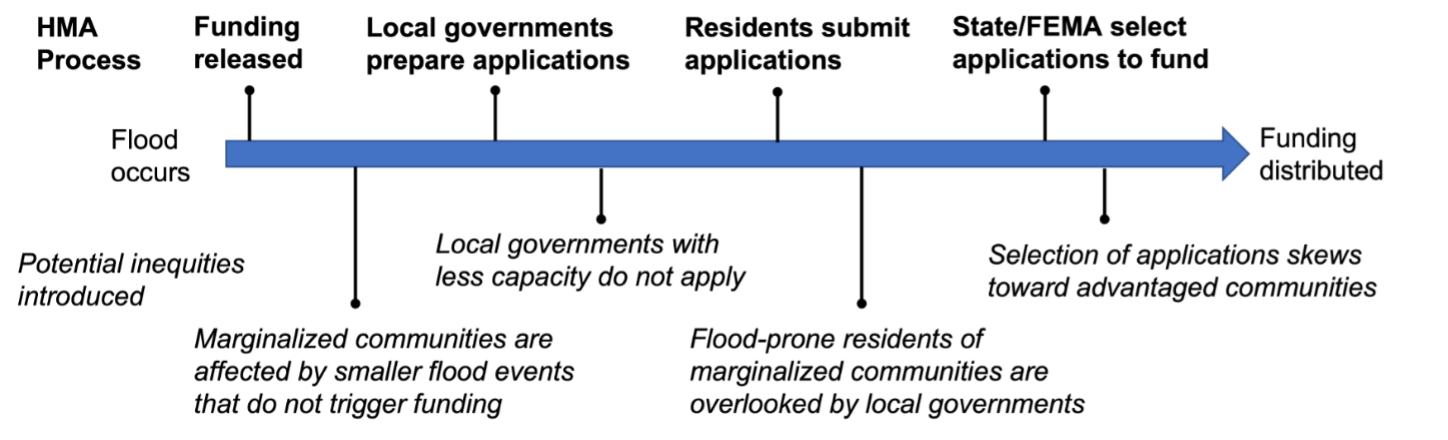
\includegraphics[keepaspectratio]{figures/Fig1_Funding_Pipeline.png}}

}

\caption{\label{fig-funding-pipeline}The application process for FEMA
Hazard Mitigation Assistance funding presents different barriers to
access at each stage. Diagram shows a simplified set of stages from
flooded to funded (top), and the associated ways in which potentially
inequitable outcomes could arise at each stage (bottom).}

\end{figure}%

\subsection{Access to federal funding for climate
resilience}\label{access-to-federal-funding-for-climate-resilience}

The federal government is the primary source of public assistance for
disaster risk mitigation, post-disaster relief, and long-term recovery
in the United States. Many federal agencies contribute to these efforts,
including the US Army Corps of Engineers (which is responsible for
large-scale flood-control infrastructure), the Department of Housing and
Urban Development (which administers Community Development Block Grant
Disaster Recovery funds), the National Oceanic and Atmospheric
Administration, and the Environmental Protection Agency. We focus our
analysis on the Federal Emergency Management Agency (FEMA), which leads
disaster response and administers the nation's largest hazard mitigation
grants. These programs --- delivered through FEMA's Hazard Mitigation
Assistance (HMA) framework --- include the post-disaster Hazard
Mitigation Grant Program (HMGP), which is triggered by presidential
disaster declarations (PDDs); Flood Mitigation Assistance (FMA), an
annually appropriated program targeting flood-insured properties; and
Building Resilient Infrastructure and Communities (BRIC), a competitive
pre-disaster program that replaced Pre-Disaster Mitigation (PDM) in
2020. FEMA made over \$1.6 billion available through BRIC and FMA alone
in FY2024, with demand for these competitive funds regularly exceeding
the available pool.

Concerns about equitable access to FEMA assistance in the aftermath of
disasters have been extensively documented, where race, sex, and other
social determinants are associated with differential rates of
participation regardless of need. Following presidential disaster
declarations, FEMA's Individuals and Households Program (IHP) provides
up to approximately \$44,000 per household for temporary housing,
property repair, unemployment assistance, and other immediate needs
(\citet{fema2024ihp}). Racial and income disparities in IHP access have
been observed across a wide range of events, including the 1994
Northridge earthquake
\citep{bolinNorthridgeEarthquakeCommunitybased1998}, Hurricane Katrina
\citep{kamelSocialMarginalisationFederal2012}, Hurricane Dolly in South
Texas \citep{riveraProceduralVulnerabilityIts2022}, and the 2017 Thomas
Fire \citep{mendezInvisibleVictimsDisaster2020}. More broadly, studies
find that social vulnerability is inversely associated with access to
federal disaster recovery funds even after accounting for the extent of
damage
\citep{emrichAssessingDistributiveInequities2022, drakesSocialVulnerabilityShortTerm2021, wilsonFloodRecoveryOutcomes2021, bentoRaciallyUnequalImpacts2022}.

Similar concerns have emerged around FEMA's risk mitigation programs,
which fund long-term adaptation rather than immediate recovery. Typical
Hazard Mitigation Assistance (HMA) projects include home elevations,
property buyouts, and community-scale infrastructure; since 2020, the
BRIC program has expanded community-wide project funding. Among
property-scale programs, buyouts have received the most scrutiny. In a
buyout, homeowners sell flood-prone properties to local governments,
which demolish structures and restore the land to open space. Initiated
in 1985 and now totaling over 43,000 completed transactions nationally,
the buyout program has shifted from its rural origins into an
increasingly urban policy \citep{machManagedRetreatVoluntary2019}. Its
geographic distribution is deeply uneven: states with the highest
cumulative flood losses (total dollars) account for comparatively few
buyouts (number of properties acquired), while nationally, buyout
activity concentrates in wealthier, denser counties with greater
administrative capacity \citep{machManagedRetreatVoluntary2019}. Within
those counties, bought-out properties are concentrated in lower-income
and more racially diverse neighborhoods, a pattern Mach et al.
\citeyearpar{machManagedRetreatVoluntary2019} describe as a ``buyout
paradox'' in which government capacity governs access at the county
scale while within-county selection follows a different logic
\citep{elliottRacialInequitiesFederal2020a, loughranUnequalRetreatsHow2022}.
By contrast, reporting on FEMA elevation grants suggests that funding
may flow disproportionately toward high-income and predominantly white
communities \citep{frankFEMAHomeElevation2022}.

\subsection{Procedural challenges to accessing
funding}\label{procedural-challenges-to-accessing-funding}

While these program-level barriers shape outcomes at a broad scale, the
mechanisms that produce inequity operate at the level of specific
program rules and local implementation practices. The HMA application
process is lengthy and multi-layered. After federal funding is released,
state, tribal, and local governments identify eligible properties,
assist homeowners in compiling required documentation (including
cost-benefit analyses, insurance records, and title documentation), and
submit project proposals. Local governments (``sub-applicants'') forward
proposals to the state (``applicant''), which screens projects before
submitting to FEMA for final review. For HMGP-funded buyouts, the full
process from disaster declaration to project closeout averages nearly
six years \citep{machManagedRetreatVoluntary2019}. The federal
government typically covers 75\% of project costs, with states, local
governments, and in some cases homeowners responsible for the remaining
25\% non-federal match. Higher federal shares apply in specific
circumstances --- up to 90\% for small, lower-income communities across
programs, and, under FMA, up to 90\% for Repetitive Loss and 100\% for
Severe Repetitive Loss properties.

Inequities can arise at every stage. At the local government level,
administrative capacity is the primary bottleneck: governments with
dedicated staff, prior grant experience, and stronger institutional
networks are far more effective at developing and submitting competitive
proposals
\citep{machManagedRetreatVoluntary2019, junodEquitableInvestmentsResilience2021a}.
At the community and household level, outreach practices vary widely;
some local governments proactively contact eligible residents and guide
them through the application process, while others do little or nothing,
effectively limiting access to only those homeowners already aware of
the program. Providing the 25\% non-federal cost share can also be a
barrier. In some states, including North Carolina, the state government
covers the matching share for HMGP buyout projects under disaster
declarations \citep{ncdpsHazardMitigationGrant2026}. Where the state
does not, the match must come from local government budgets or
individual homeowners --- and sometimes from community organizations or
nonprofits, though we do not observe these contributions in our data.
Reliance on these sources can significantly constrain participation
among cash-strapped jurisdictions and lower-income households.

At the household level, procedural requirements such as documentation,
inspections, and legal title verification can impose substantial
compliance burdens. While these requirements apply uniformly to
applicants, the practical difficulty of meeting them is likely to vary
systematically with household resources, mirroring documented patterns
in IHP access
\citep{riveraProceduralVulnerabilityIts2022, rakerStratifyingDisasterState2023}.
Finally, federal cost-benefit analysis (CBA) requirements may further
filter the pool. CBA evaluates projects on a benefit-to-cost ratio in
which avoided losses scale with property replacement value, leading to
concerns that applications from lower-value properties could face
systematic disadvantages in the benefit-to-cost ratio
\citep{tateFloodExposureSocial2021, junodEquitableInvestmentsResilience2021a, millerCostCostEffectivenessExpanding2023}.
This expectation is complicated, however. Project costs also rise with
property value, and some projects (i.e.~acquisitions of substantially
damaged homes, or any project under \$1 million) can qualify as
cost-effective without a property-specific benefit-cost analysis,
relying instead on pre-calculated benefits or a simplified written
justification
\citep{femaHMAProgramPolicyGuide2024, femaBCAStreamlined2024}. Whether
CBA, on net, pushes funded properties toward higher or lower property
values therefore remains an open empirical question.

\section{Results}\label{results}

We track 3.14 million residential parcels across 78 counties in eastern
North Carolina through four sequential stages of the federal HMA
pipeline: flooded (intersection with any of 78 modeled flood-event
footprints from 1996 through 2020), in an applying community
(jurisdiction with at least one HMA application submitted during the
study period), applied (parcel itself named on an HMA application), and
funded (application ultimately awarded). Flood-exposure data come from
flood extent maps created using random forest models trained on NFIP
claims and policies-in-force
\citep{garciaReconstructingRepetitiveFlood2025}, application and funding
records from the North Carolina Department of Public Safety, and
neighborhood demographics from the 2013 American Community Survey at the
block-group scale. Property values come from the CoreLogic database and
are expressed as percentile ranks across the study-area sample. Detailed
methods are described in the Materials and Methods section.

\begin{figure}

\centering{

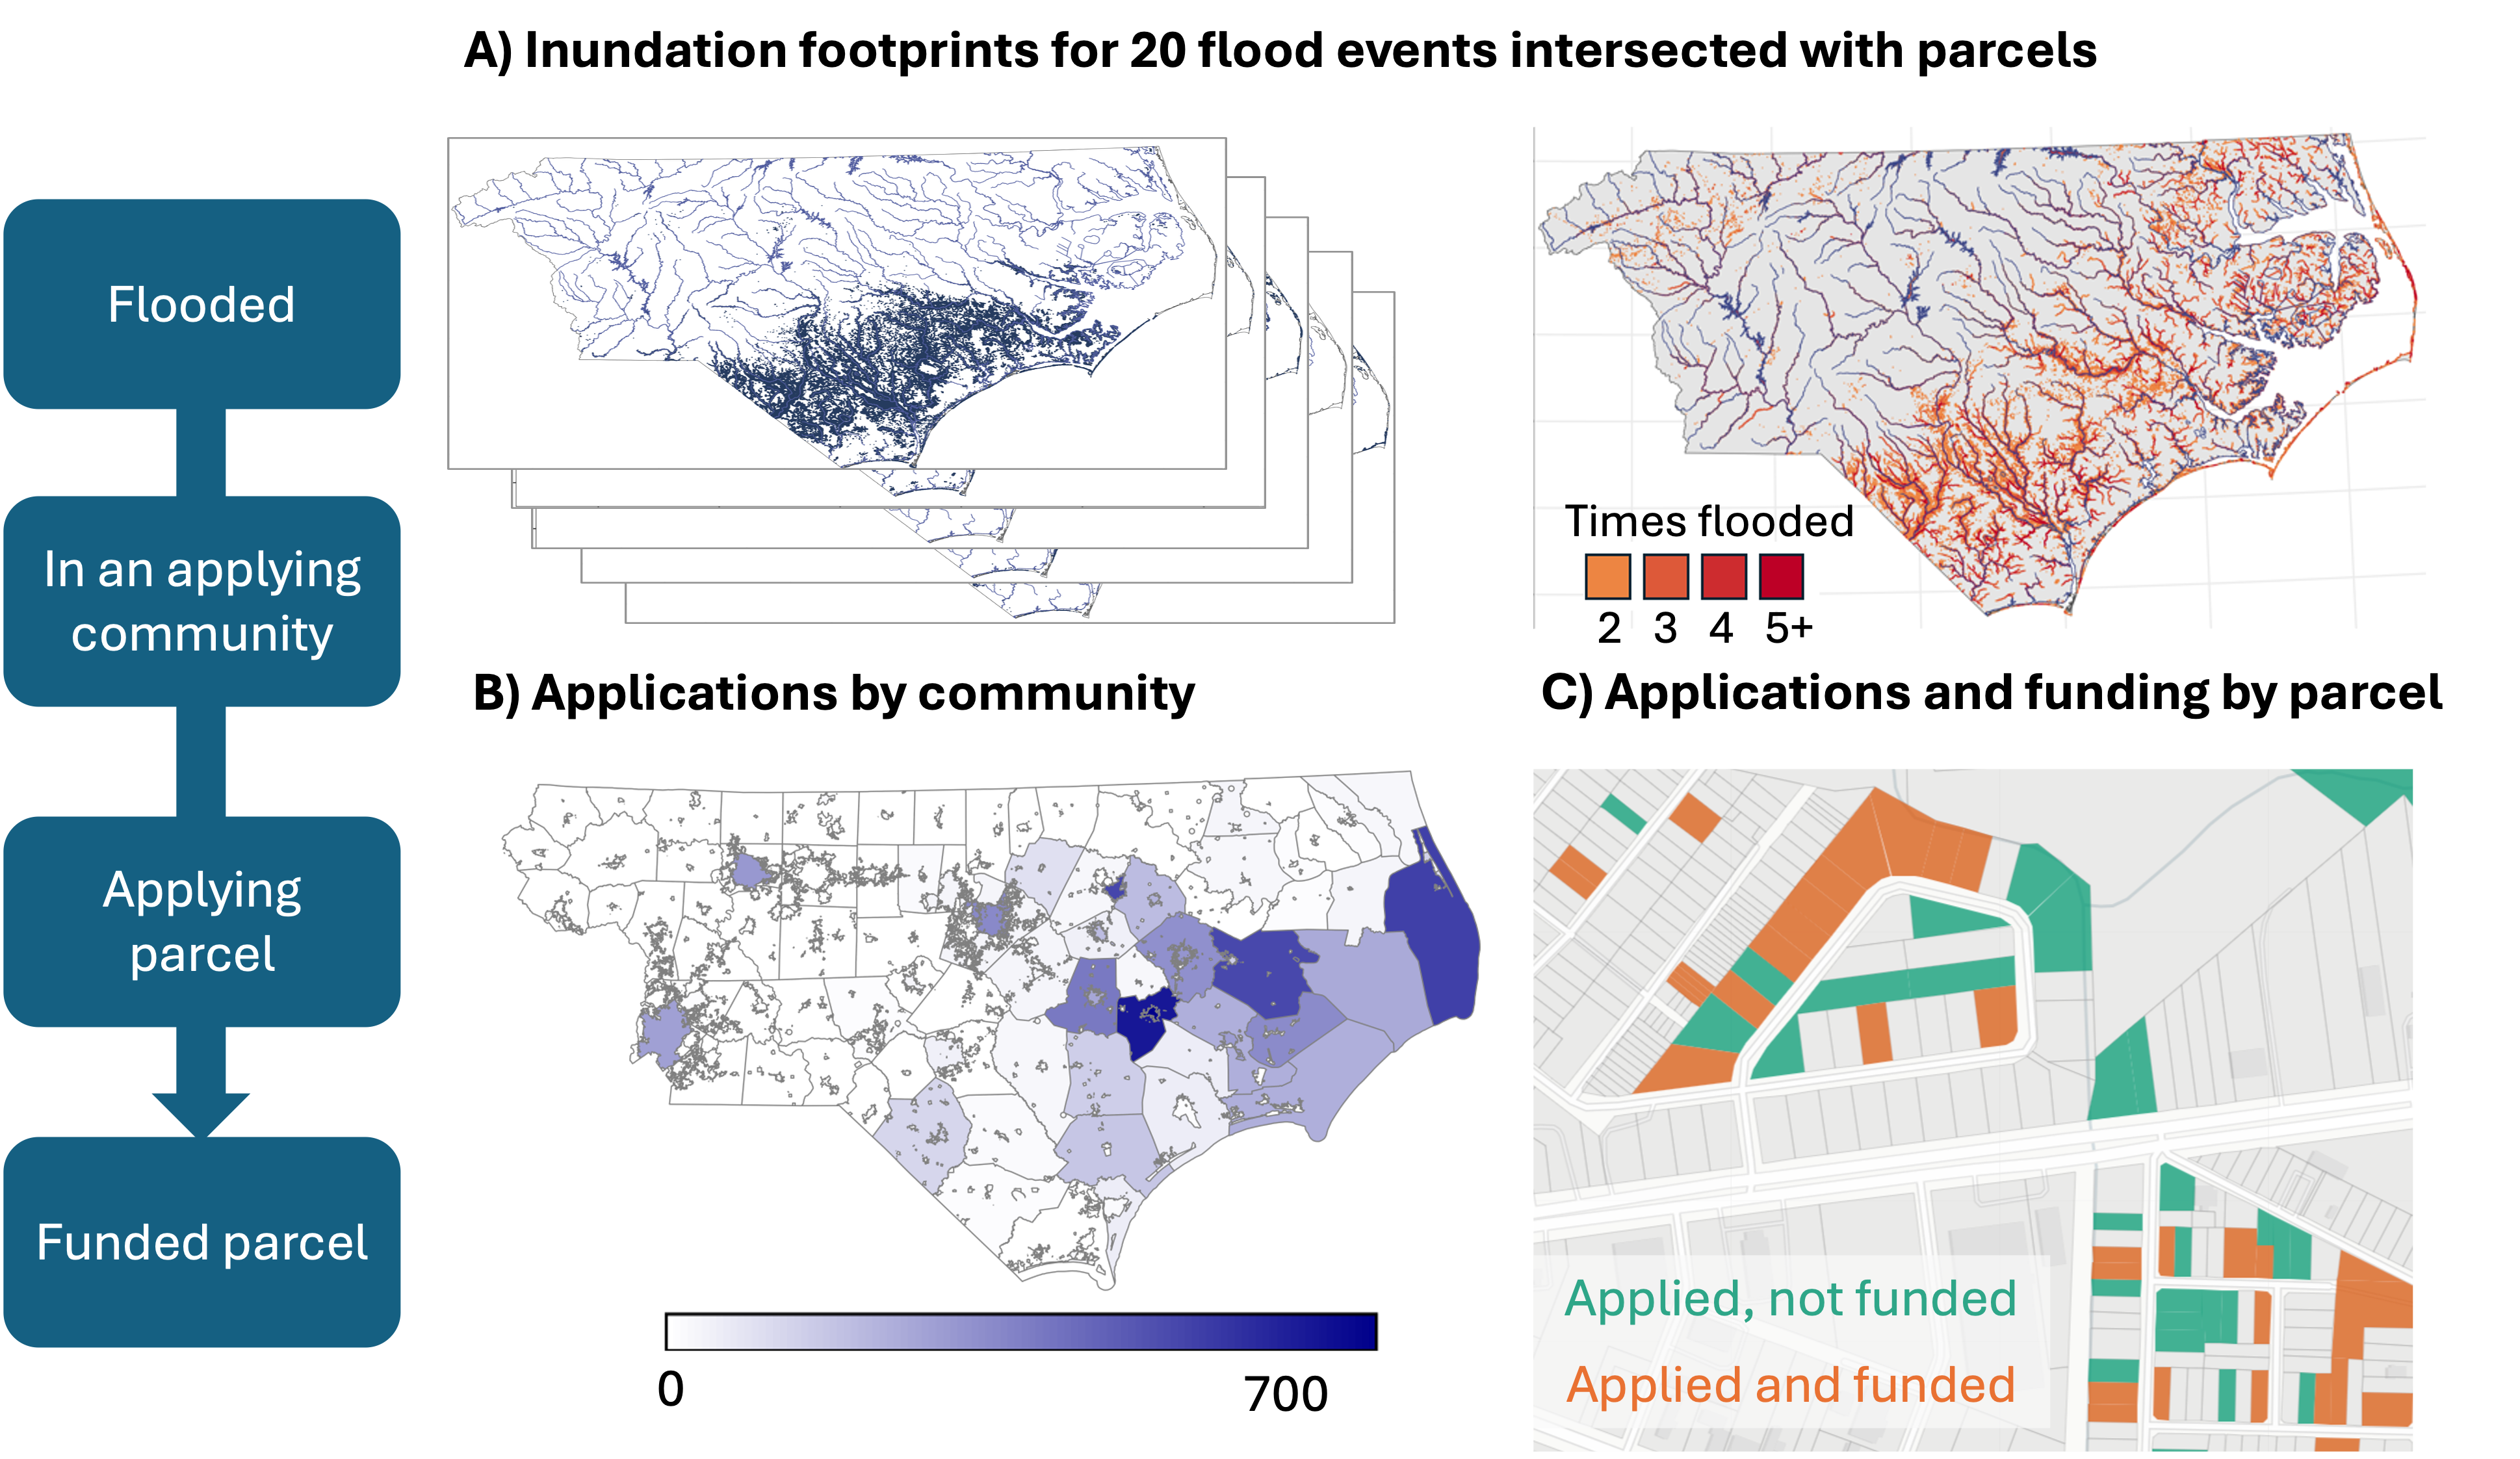
\includegraphics[width=1\linewidth,height=\textheight,keepaspectratio]{figures/Fig2_Pipeline.png}

}

\caption{\label{fig-data}\textbf{Spatial distribution of properties
across the flooded-to-funded pipeline.} Left: schematic of the four
sequential pipeline stages tracked in our analysis. Top-left: flooded
parcels (n = 202,623) across the 78-county study area, with stacked
footprints from 78 modeled flood events between 1996 and 2020.
Top-right: repetitive residential flooding, with cells colored by the
number of modeled flood events affecting each location (2, 3, 4, or 5+
events). Bottom-left: jurisdictions classified as applying communities
(shaded by share of eligible parcels named on at least one HMA
application). Bottom-right: representative neighborhood showing
individual parcels named on HMA applications, distinguished by funding
outcome (applied but not funded vs.~applied and funded).}

\end{figure}%

Among all flooded properties (Figure~\ref{fig-funnel}, Panel A), 65.6\%
are in jurisdictions where the local government submitted at least one
HMA application, yet only 2.8\% apply themselves. Of those that apply,
59.7\% are funded --- just 1.7\% of all flooded properties. The steepest
attrition occurs at the application step, not at community participation
or funding selection.

Approximately 32.8\% of flooded properties were exposed to more than one
of the 78 modeled events (Figure~\ref{fig-funnel}, right panel).
Repeat-flooded properties are more likely to be located in jurisdictions
with at least one HMA application (81.1\% versus 65.6\% among all
flooded properties) and apply at roughly twice the rate of once-flooded
properties (5.6\% versus 2.8\%). However, the share of applications that
ultimately receive funding is essentially the same across the two groups
(58.5\% versus 59.7\%), indicating that while greater flood exposure
increases the likelihood of applying, it does not appear to influence
selection likelihood among those who do apply.

\begin{figure}

\centering{

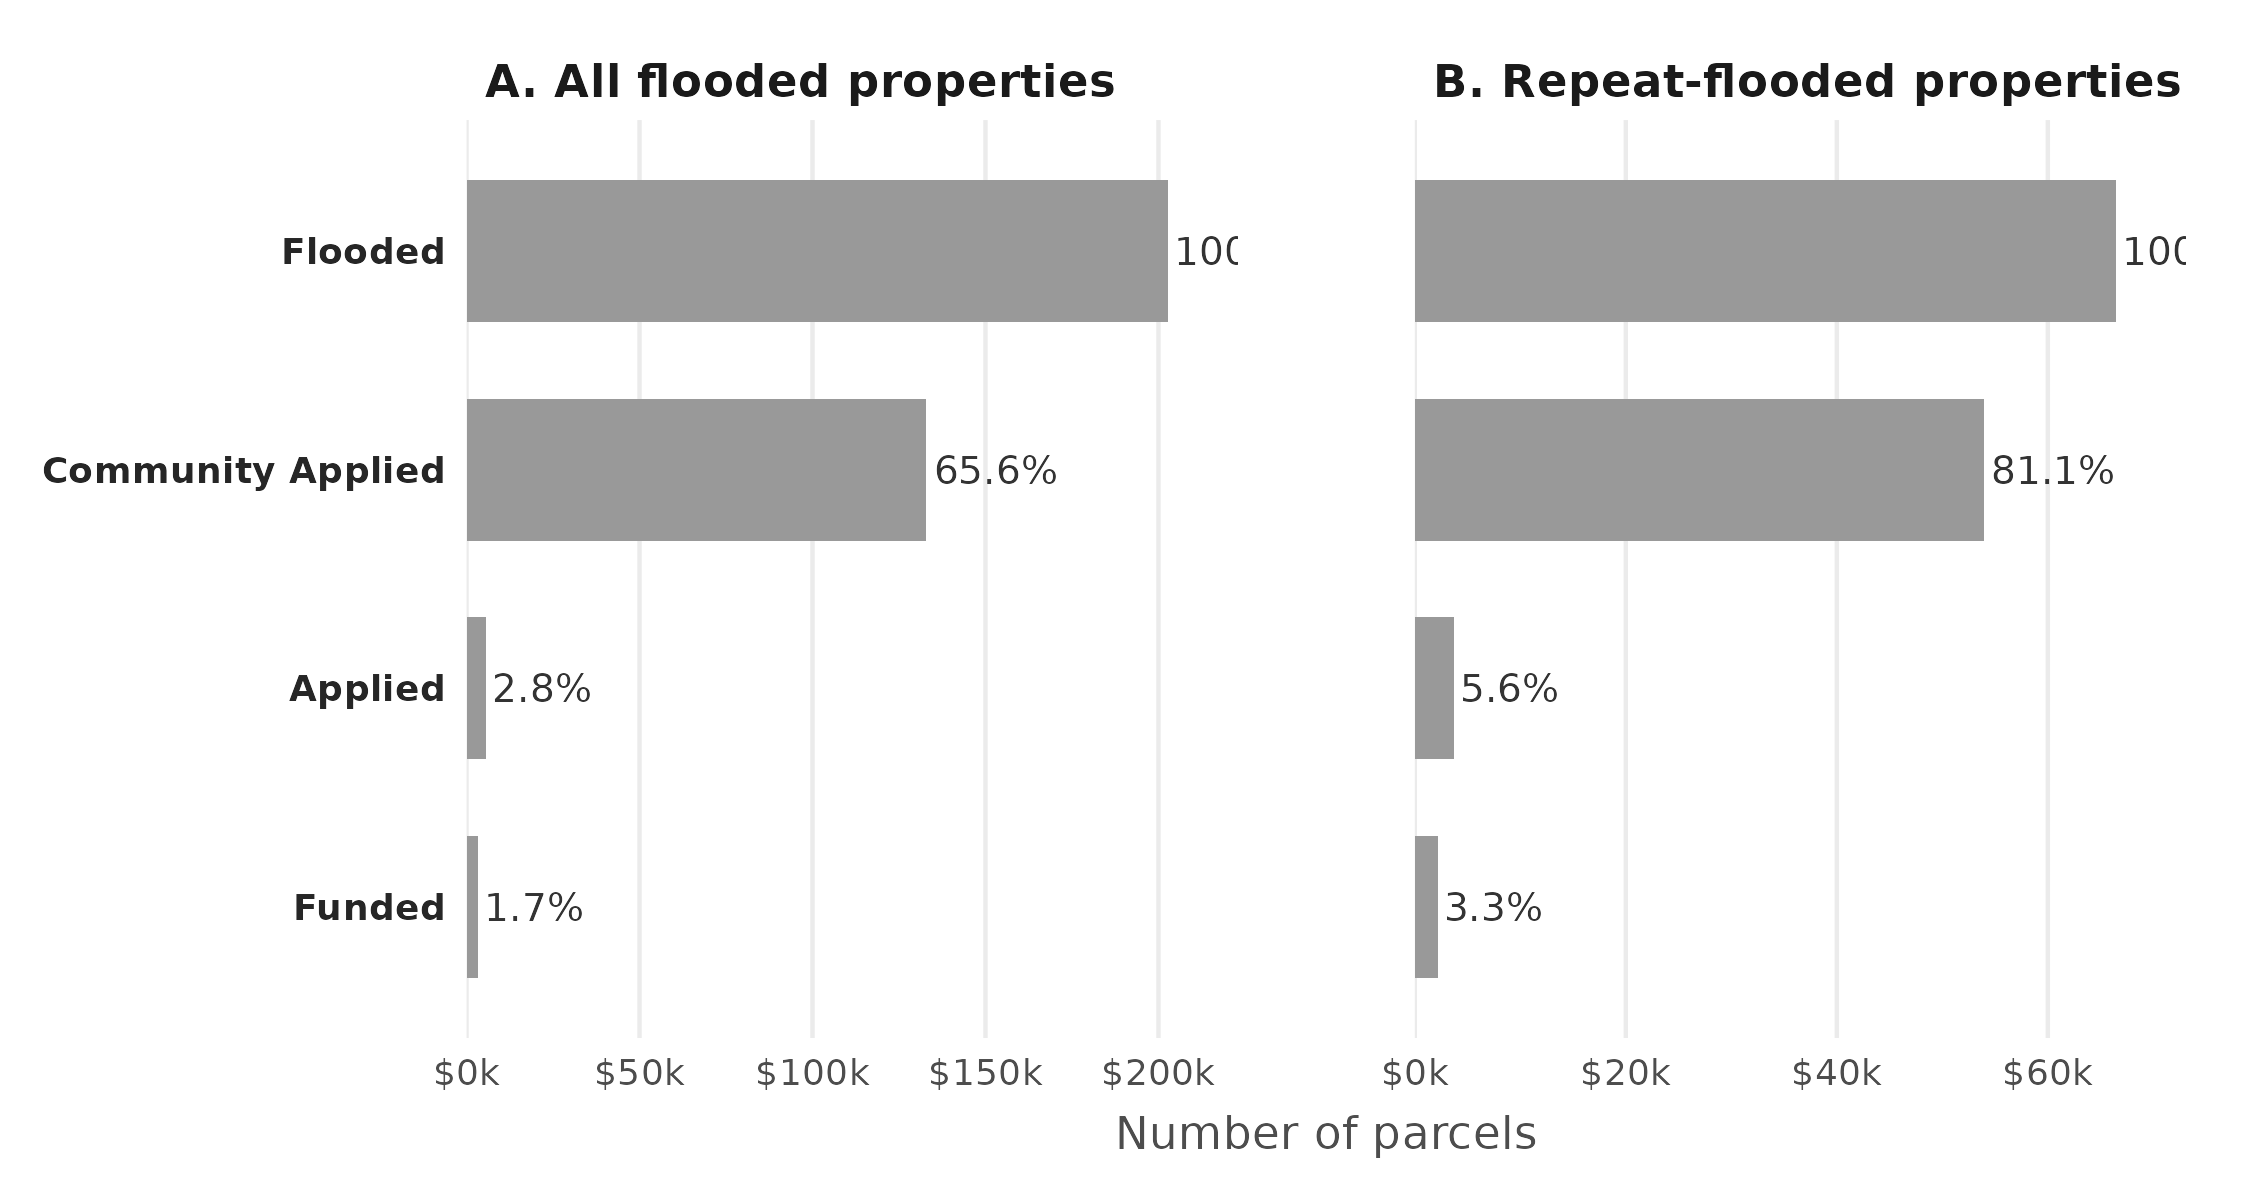
\includegraphics[width=1\linewidth,height=\textheight,keepaspectratio]{figures/fig2.png}

}

\caption{\label{fig-funnel}\textbf{The application stage is the largest
attrition point in the HMA pipeline: fewer than 3\% of flooded
properties ever submit an application.} Bars show the number of 1--4
family residential parcels at each of four pipeline stages: flooded in
any of the 78 modeled events; in an applying community (jurisdiction
with at least one HMA application during the study period); itself named
on an HMA application; and ultimately funded. Panel A: all flood-exposed
parcels (n = 202,623). Panel B: parcels exposed to flooding in more than
one event (n = 66,443). Repeat-flooded properties apply at roughly twice
the rate of once-flooded properties but are funded at similar rates.}

\end{figure}%

\begin{figure}

\centering{

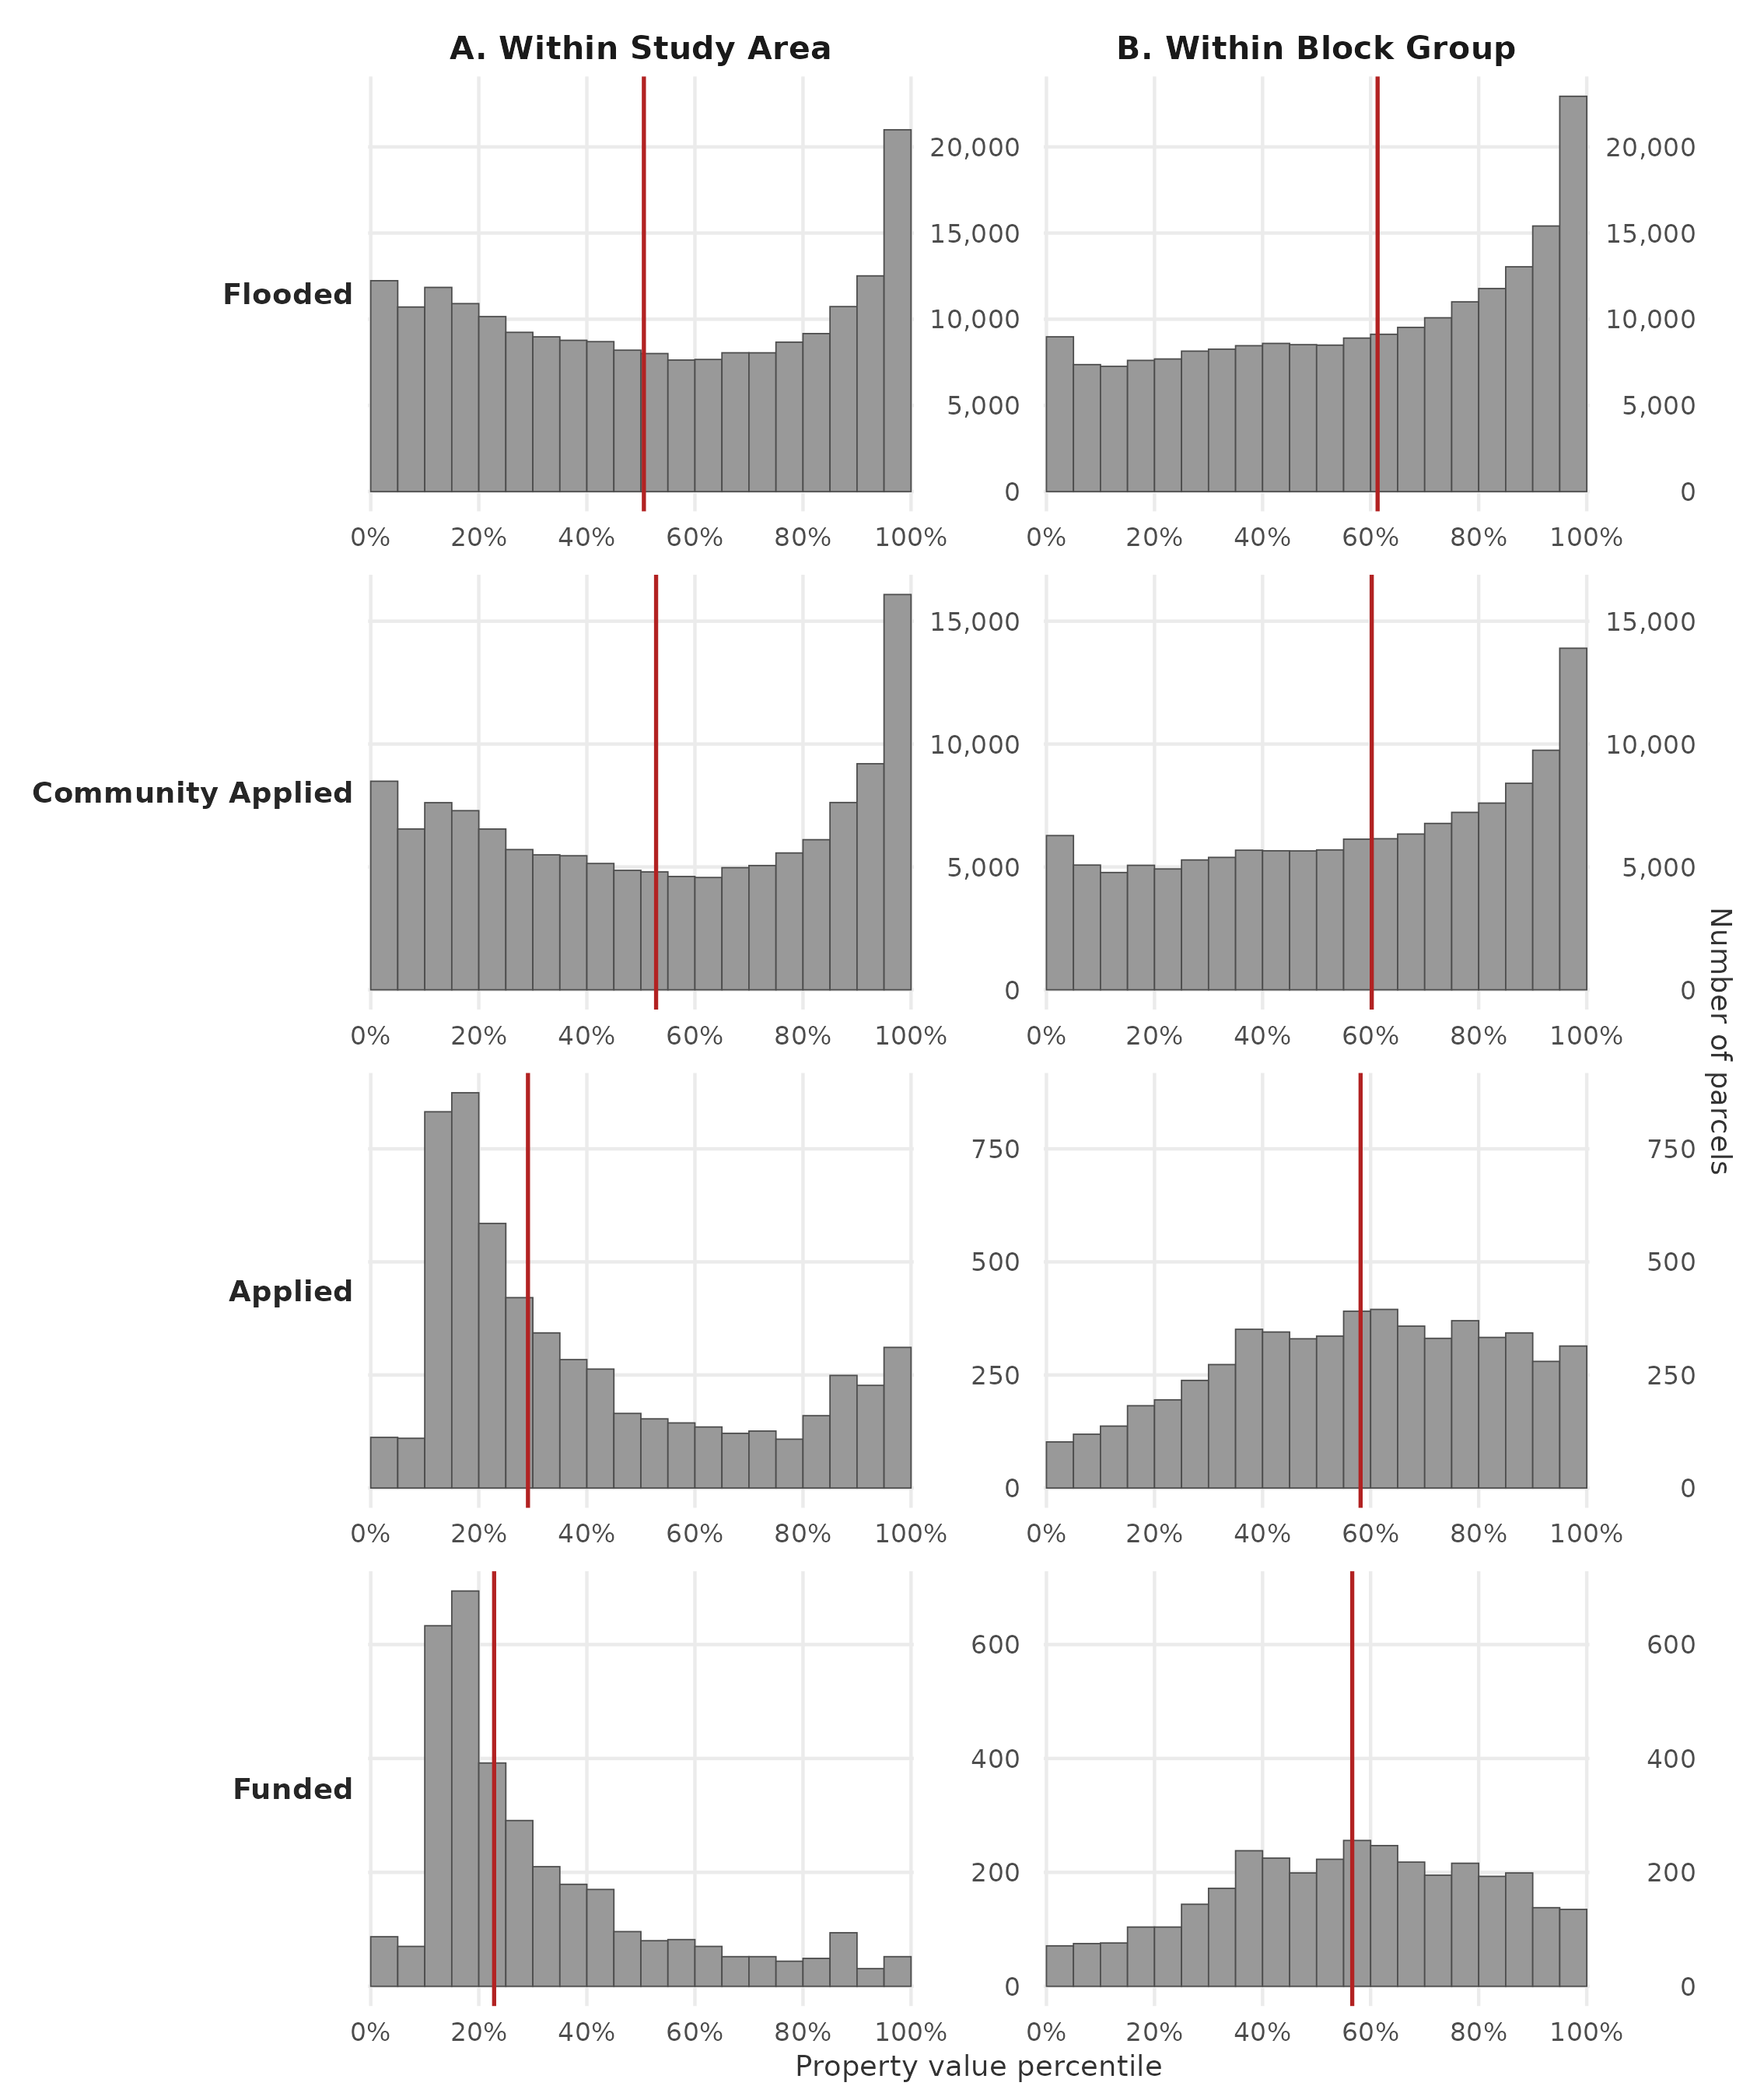
\includegraphics[width=1\linewidth,height=\textheight,keepaspectratio]{figures/fig3.png}

}

\caption{\label{fig-value}\textbf{Funded properties are lower-value than
the broader flood-exposed population, but are not the lowest-value homes
within their own neighborhoods.} (A) Distribution of property values for
parcels reaching each stage of the flooded-to-funded pipeline, expressed
as percentile ranks relative to the entire study-area sample. (B) The
same distributions, expressed as percentile ranks within each parcel's
block group. Property values are from CoreLogic (2022 dollars); red
vertical lines mark stage medians.}

\end{figure}%

Property values shift substantially across pipeline stages, both
relative to the broader study area and within each property's own block
group (Figure~\ref{fig-value}). Properties that flooded or that reside
in communities with at least one HMA application have median values near
the 51th--53th percentile of the study-area sample (Panel A). The median
value for properties that apply for funding drops to the 29th
percentile, and the median for those that are funded is even more
affordable at the 23rd percentile. Panel B re-ranks each property
against other parcels in its own block group, with all stages clustering
near the 60th percentile (Flooded: 61st, Funded: 57th). The much larger
spread in Panel A, where flooded properties are within the 51st
percentile and funded properties at the 23rd, indicates that the
property-value shift across pipeline stages is driven by selection
between neighborhoods rather than within them. Funded properties are not
the lowest-value homes in their neighborhoods --- they sit slightly
above the local median (around the 57th percentile), a position that
changes little across pipeline stages. Two-sample Kolmogorov--Smirnov
tests echo this contrast: the property-value distribution shifts
substantially between the flooded and funded stages relative to the
study area (D = 0.342) but much less within block groups (D = 0.126).
The shift toward lower-value properties therefore operates between
neighborhoods rather than within them.

\begin{figure}

\centering{

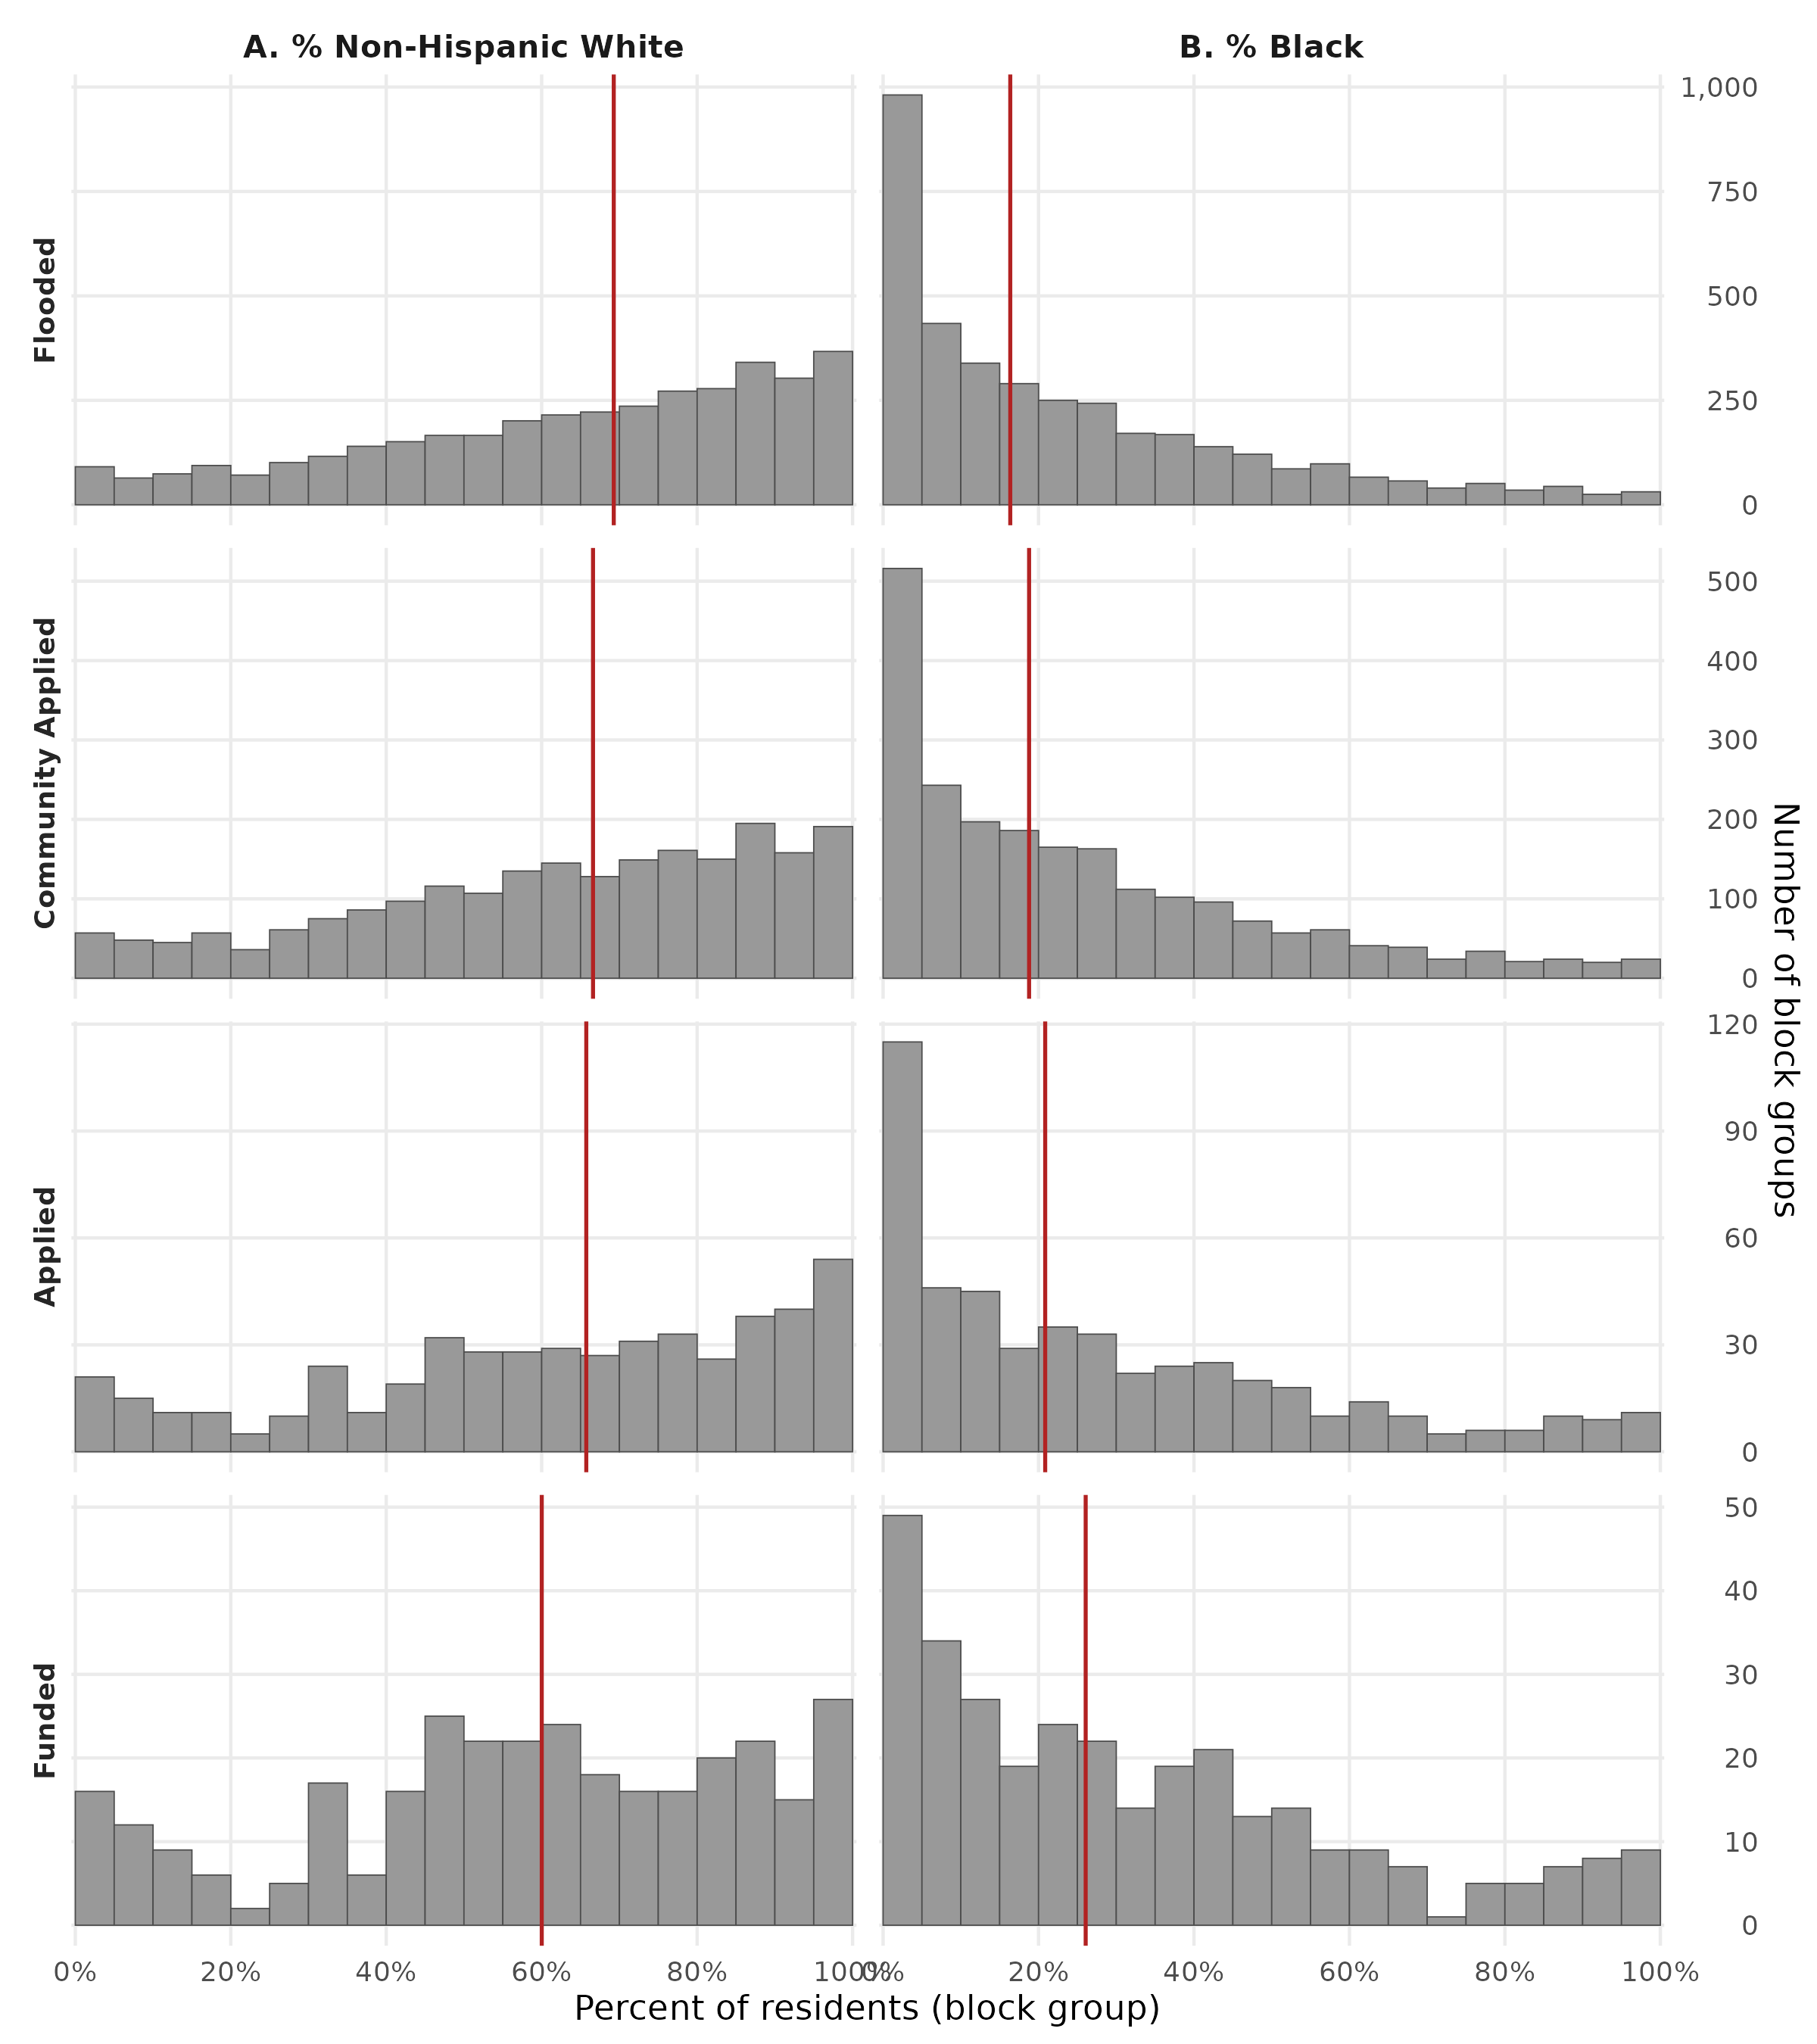
\includegraphics[width=1\linewidth,height=\textheight,keepaspectratio]{figures/fig4.png}

}

\caption{\label{fig-race}\textbf{Funded properties are more likely to be
in less-white, more-Black neighborhoods than the broader flood-exposed
population.} (A) Percentage of non-Hispanic White residents. (B)
Percentage of Black residents. One observation per block group
containing ≥ 1 residential parcel reaching the stage; demographic data
from the 2013 ACS 5-year estimates. Red vertical lines mark stage
medians.}

\end{figure}%

Properties applying for and receiving mitigation funding are located in
block groups with lower shares of non-Hispanic White residents and
correspondingly higher shares of Black residents than block groups at
preceding pipeline stages (Figure~\ref{fig-race}). Two-sample
Kolmogorov--Smirnov tests show that the block-group racial-composition
distributions shift substantially between the flooded and funded stages
(NH White: D = 0.131; Black: D = 0.151). Median NH White share declines
from 69.3\% at the flooded stage to 60.0\% at funded properties, with a
near-symmetric rise in Black share from 16.4\% to 26.1\%.

The racial composition of funded parcels differs substantially by
mitigation type (Figure~\ref{fig-mit-type}), which contributes to the
funded-stage shift documented in Figure~\ref{fig-race}. Among funded
parcels with a classified project type, buyouts outnumber elevations by
approximately 4:1 (1,879 buyouts vs 415 elevations). Buyouts sit in
block groups with substantially higher shares of Black residents than
elevations (median 47\% versus 35.7\%; Kolmogorov--Smirnov D = 0.366, p
\textless{} 0.001). By contrast, the two types occupy similarly valued
properties --- their property-value distributions largely overlap
(median 20th versus 25.7th percentile; D = 0.141, p \textless{} 0.001).
The buyout--elevation difference in racial composition also holds among
repeat-flooded funded parcels (D = 0.32), so it is not confined to
once-flooded properties. Because roughly one-third of funded parcels
have project types we could not classify, we cannot fully attribute the
Figure~\ref{fig-race} shift to either mechanism, but buyouts' higher
prevalence and their concentration in less-white neighborhoods suggest
they are a meaningful contributor.

\begin{figure}

\centering{

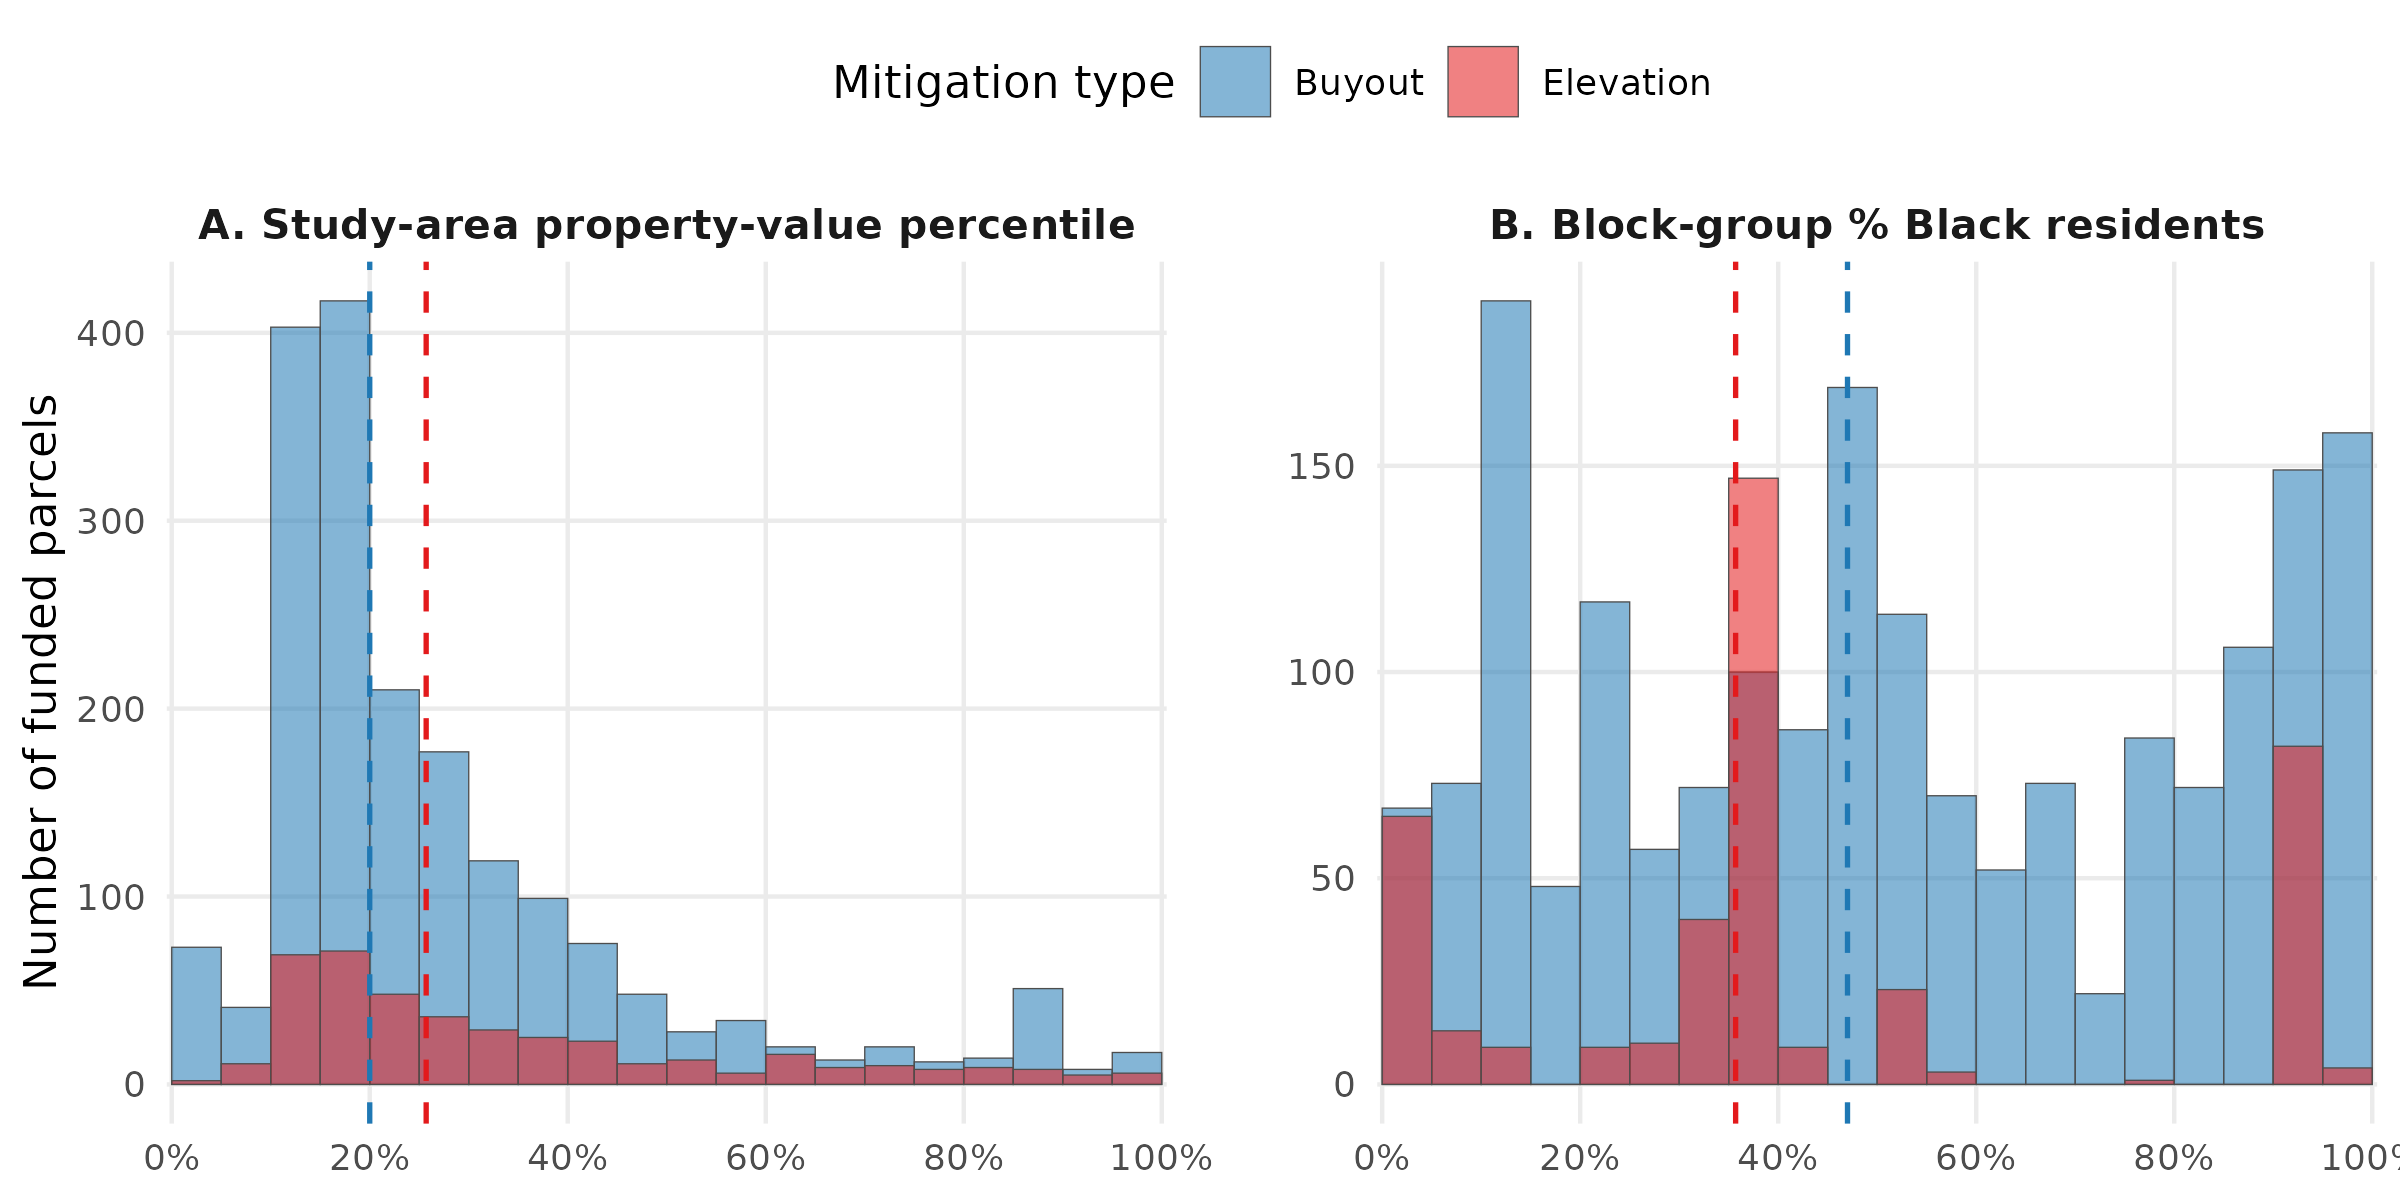
\includegraphics[width=1\linewidth,height=\textheight,keepaspectratio]{figures/fig5_mit_type.png}

}

\caption{\label{fig-mit-type}\textbf{The racial-composition shift at the
funded stage is driven by buyouts.} Distributions of (A) study-area
property-value percentile rank and (B) block-group share of Black
residents, comparing funded parcels classified as buyouts (blue) and
elevations (red); dashed vertical lines mark each group's median. Within
each panel, a two-sample Kolmogorov--Smirnov test compares the buyout
and elevation distributions, where D is the maximum distance between
their cumulative distributions (0 = identical, 1 = fully separated).
Buyouts and elevations differ sharply in neighborhood Black share (Panel
B: D = 0.366, p \textless{} 0.001) but overlap in property value (Panel
A: D = 0.141, p \textless{} 0.001). Funded parcels without a recorded
project-type classification (approximately one-third of the funded set)
are excluded.}

\end{figure}%

\section{Discussion}\label{discussion}

Our analysis identifies the application stage as the critical pinch
point in the flooded-to-funded HMA pipeline. Of all flooded residential
properties in eastern North Carolina, only 2.8\% apply for funding, and
of those, 59.7\% receive an award. By tracking the full population of
flooded properties rather than only those that received funding, we
identify a substantial population of households --- to our knowledge not
previously quantified at the property scale --- that would benefit from
mitigation assistance but never enter the applicant pool. This
unrealized demand suggests that interventions targeting the application
stage may do more to expand the reach of funding to flooded households
than refining the selection criteria applied to the small pool of
existing applicants.

Many of these non-applying properties have flooded repeatedly. Because
repeatedly flooded properties carry higher expected avoided losses ---
and thus more readily clear federal benefit-cost thresholds --- yet are
funded at no higher a rate than other applicants, directing outreach
toward these households could raise the average cost-effectiveness of
the funded portfolio, which refining selection among existing applicants
cannot achieve. Fully capturing the unmet demand we document, however,
would require additional mitigation appropriations rather than
reallocation of a fixed budget, since demand already exceeds available
funding.

Among the small fraction of properties that receive funding, the
composition shifts toward lower-value, less-white neighborhoods.
Relative to the flooded stage, funded properties fall at the 23rd
percentile of the study-area property-value distribution (from the
51st), sit in block groups with a median non-Hispanic white share of
60\% (from 69.3\%) and a median Black share of 26.1\% (from 16.4\%).
This shift occurs primarily between neighborhoods rather than within
them: within-block-group percentiles for funded properties differ only
modestly from those at the flooded stage. The racial shift likely tracks
the value shift through the strong correlation between race and property
value in eastern North Carolina, where less-white neighborhoods tend to
be lower-value (Figure~\ref{fig-si-race-value}). This neighborhood-scale
pattern aligns with prior work
\citep{machManagedRetreatVoluntary2019, elliottRacialInequitiesFederal2020a},
which finds that within whiter, wealthier counties funding concentrates
in lower-value, less-white neighborhoods; because we do not conduct an
analogous county-level comparison, our results speak to this
within-county scale rather than the county-scale pattern those studies
also document.

That funding reaches these lower-value, less-white neighborhoods
indicates applicants from them are not disadvantaged at the selection
stage --- the inequity we identify arises earlier, at application.
Whether the shift is itself equitable is a separate question, however,
particularly for buyouts, where funding concentrated in lower-income,
less-white neighborhoods may reflect the disproportionate relocation of
marginalized residents rather than an equitable distribution of benefit.

Repeat-flooded properties apply at roughly twice the rate of
once-flooded properties but are funded at similar rates. This pattern
suggests that flood-exposure history influences application behavior
more than selection outcomes, and points to an underused targeting lever
for HMA prioritization. HMGP, which dominates HMA funding in our study
area, becomes available event-by-event following PDDs and weights damage
from a single event heavily in the cost-benefit calculation. Mitigation
programs that weighted cumulative flood history over single-event
severity would concentrate funding where expected avoided losses, and
thus cost-effectiveness, are greatest.

Decomposing the funded set by mitigation type shows that the
racial-composition shift at the funded stage is a buyout phenomenon
(Figure~\ref{fig-mit-type}). Buyouts sit in block groups with a
substantially higher median Black share than elevations (47\%
vs.~35.7\%; KS D = 0.366, p \textless{} 0.001;
Figure~\ref{fig-mit-type}, Panel B). By contrast, the property-value
distributions of buyouts and elevations largely overlap (D = 0.141, p
\textless{} 0.001), so the property-value shift across the pipeline
reflects a neighborhood-scale selection process affecting both
mitigation types similarly, whereas the racial-composition shift is
buyout-specific. This parcel-scale, within-neighborhood pattern extends
prior county-scale findings of demographic differences between buyout
and elevation targeting
\citep{machManagedRetreatVoluntary2019, elliottRacialInequitiesFederal2020a, frankFEMAHomeElevation2022}.
The gap is not confined to once-flooded properties: among repeat-flooded
funded parcels, buyouts still fall in markedly more-Black block groups
than elevations (D = 0.32, p \textless{} 0.001), consistent with a
systematic difference in how the two programs are sited.

Our cross-sectional data also let us rule out several candidate
mechanisms for the equity patterns we observe. If the federal CBA
requirement were primarily driving selection toward higher-value
properties, we would expect funded properties to be concentrated at
higher property values; instead, we see the opposite, and many
lower-value properties apply. This holds within neighborhoods as well
where funded properties sit only slightly above their block-group median
(\textasciitilde60th percentile, roughly the same position they occupy
at the flooded stage) so funding shows no tendency to select
higher-value homes even within a given neighborhood. Because CBA is a
federal rule applied uniformly across states, this pattern should
generalize beyond North Carolina. Community participation is not the
binding constraint in our study area: 65.6\% of flooded properties sit
in jurisdictions with at least one HMA application, yet only 2.8\% apply
themselves. The sharp attrition occurs at the individual application
stage, not the community stage. This likely differs in states without
North Carolina's state-level cost-share absorption, where community
participation may itself be a larger barrier. We also see no evidence of
applicant pools dominated by high-value properties, which would be
consistent with local governments selectively recruiting wealthier
households for application support, though this pattern may be specific
to North Carolina and could differ in states with different local
capacity or outreach practices. Together, these patterns suggest that
the concentration of funding in lower-value, less-white communities is
determined primarily at the application stage --- where the median shift
toward these communities is largest --- rather than by selection within
the applicant pool, where the applied-to-funded shift is comparatively
modest. In other words, the pattern appears to be a function of who
applies, and who is solicited to apply, more than which applications are
chosen. Disentangling whether this reflects differential outreach,
programmatic preferences for buyout siting, or other mechanisms is an
important direction for future work.

Several methodological limitations apply. First, our flood-exposure data
come from a reconstruction of 78 flood events in eastern North Carolina
between 1996 and 2020 \citep{garciaReconstructingRepetitiveFlood2025}.
The underlying models are conservative and likely underestimate the true
population of flood-exposed properties. A sensitivity analysis dropping
the seven events Garcia et al.~flag for unusually high
modeled-to-observed damage ratios produces materially identical headline
findings: the number of funded parcels changes by only 2.3\%, and median
demographic compositions move by less than half a percentage point
(Supplementary Materials). Second, our data on the timing of
applications and mitigations is incomplete, so we do not distinguish
between floods that occur before or after a property is funded for
mitigation. This is particularly relevant for our repeat-flood analysis:
properties that were elevated or bought out before a subsequent modeled
flood event may appear in our data as repeat-flooded even though the
structure may no longer have been exposed or may have been physically
removed. Because we do not observe the date on which each buyout or
elevation was completed, we cannot determine when a property entered its
mitigated state; rather than drop these properties on the basis of
assumptions, we conservatively retain them throughout the sample.
Because these cases require a property to have already been funded for
mitigation, they should be concentrated in the funded stage and are
unlikely to be numerous; they would, if anything, modestly overstate the
funding rate among repeat-flooded properties rather than change our
central conclusion that repeat-flooded properties apply at higher rates
but are funded at similar rates to once-flooded properties. Third,
approximately one third of funded mitigation records lack a project-type
classification, so our buyout-versus-elevation comparison
(Figure~\ref{fig-mit-type}) is restricted to the classified subset. We
cannot observe whether these unclassified records skew toward buyouts or
elevations; on the attributes we do observe, however, they closely
resemble the classified records (median value percentile 27.5 vs.~21;
median block-group Black share 34\% vs.~47\%), suggesting the missing
classifications are not strongly systematic along the dimensions central
to our findings. We nonetheless cannot rule out differences by
mitigation type itself, which we do not observe. Fourth, our block-group
demographic data come from the 2013 American Community Survey, which
falls near the midpoint of the study window but does not capture
demographic changes over the full 1996--2020 period. Finally, while we
document more of the application process than past studies, there are
still many aspects that we do not observe, such as how local governments
approach (or fail to approach) flooded households about funding
opportunities, procedural obstacles that may deter applications from
interested households, and sources of non-governmental assistance.

A broader interpretive caveat concerns what our findings imply for
affected households. Federal mitigation funding flows disproportionately
to lower-value, less-white block groups relative to the broader
flood-exposed population, a pattern consistent with mitigation reaching
historically underserved communities in North Carolina. Whether
participation actually serves these households, however, requires
post-mitigation outcome data we do not have; this is particularly
relevant for buyouts, where prior research has questioned whether
participation reflects informed preference or limited alternatives
\citep{machManagedRetreatVoluntary2019}. Within block groups, funded
properties sit slightly above the local median rather than being the
lowest-value homes, so the compositional shift we observe is driven
largely by upstream pipeline stages --- community participation,
application rates, and the spatial distribution of flood exposure itself
--- rather than by the within-neighborhood selection of which properties
are ultimately funded. We do not observe within-neighborhood racial
shifts directly, since racial composition is measured only at the
block-group level; however, the stability of within-neighborhood
property-value percentiles across pipeline stages, together with the
strong neighborhood-scale correlation between race and property value,
gives us some basis to infer that little within-neighborhood racial
selection occurs. Procedural neutrality at any one step is not
sufficient to establish that the cumulative distribution of funding is
substantively equitable.

\subsection{Conclusions}\label{conclusions}

This study follows individual residential properties from flood exposure
through mitigation funding outcome at each significant stage, including
the previously unobserved application stage. The largest falloff in the
pipeline occurs at the application step, and properties that reach
subsequent stages tend to be lower-value and located in less-white
neighborhoods. For property value, this shift operates primarily between
neighborhoods rather than within them; because racial composition is
measured only at the block-group level, the racial shift is necessarily
a between-neighborhood pattern, and within-neighborhood racial selection
is something we cannot observe. These results identify two leverage
points that prior work --- focused on funded outcomes alone --- could
not observe. The first is the application stage: expanding who applies
would broaden access to federal mitigation funding. The second lies in
the funding decision itself, where repeatedly flooded applicants are
funded at no higher a rate than once-flooded applicants despite their
higher expected avoided losses; reweighting cost-benefit criteria toward
cumulative flood history offers a concrete, lower-cost way to align
funding with risk.

These findings arrive amid significant federal restructuring of hazard
mitigation policy. The FEMA Review Council's May 2026 final report
recommended replacing HMGP with a state-managed Refined Risk Reduction
Program that would prioritize repetitively flooded properties and
acknowledged administrative burdens that may discourage applications
from under-resourced communities \citep{femaReviewCouncilFinal2026}. The
application-stage attrition we document is consistent with those
concerns. Reforms targeting funding-side changes such as disbursement
speed, federal priority-setting, or program structure will require
complementary attention to application-stage barriers if they are to
translate into broader access. Future research could extend this
approach to community-scale infrastructure investments such as
stormwater system upgrades and BRIC community projects, which may also
reduce household-level flood risk through complementary pathways.

\section{Methods}\label{methods}

We assemble over 20 years of data on flood exposure, applications for
state and federal funding, and funding allocations. Flood exposure data
are generated using a random forest model trained on address-level
records of National Flood Insurance Program (NFIP) policies-in-force and
claims filed from January 1996 through September 2020, obtained from
FEMA Region IV \citep{garciaReconstructingRepetitiveFlood2025}. The
model domain encompasses the entirety of the Neuse--Pamlico and Cape
Fear watersheds and portions of the Pee Dee and Chowan--Roanoke
watersheds that drain through eastern North Carolina, overlapping with
78 of North Carolina's 100 counties (Figure~\ref{fig-studyarea}). This
measure indicates whether a parcel intersected the modeled footprint of
an event but does not capture the severity of any individual exposure;
some properties classified as flooded may have experienced relatively
minor inundation. We link these flood exposure data to parcel geometries
from the North Carolina OneMap database, attribute records from the
CoreLogic property database, application and funding records from the
North Carolina Department of Public Safety (NCDPS), and block-group
demographic data from the American Community Survey (ACS).

\phantomsection\label{cell-fig-studyarea}
\begin{figure}[H]

\centering{

\pandocbounded{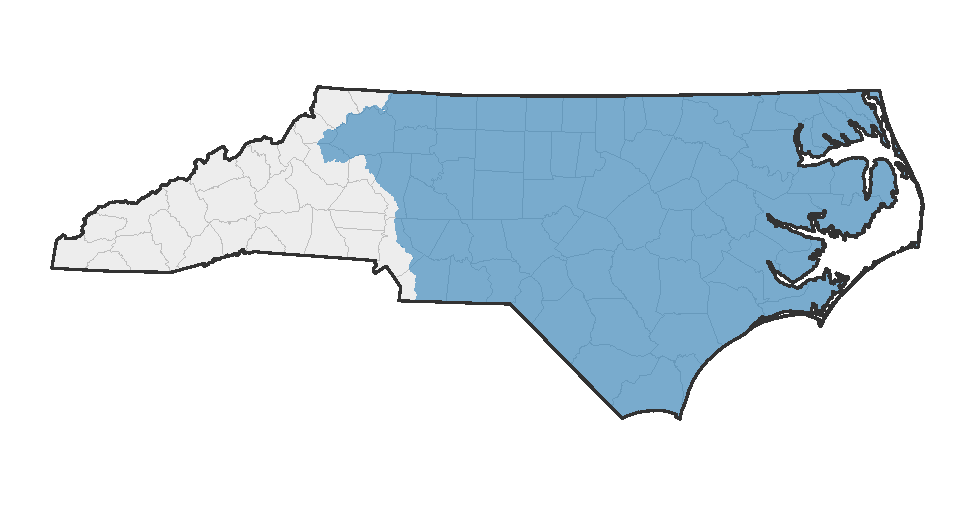
\includegraphics[keepaspectratio]{index_files/figure-pdf/fig-studyarea-1.pdf}}

}

\caption{\label{fig-studyarea}Study-area domain within North Carolina.
The shaded region shows the model domain (the union of the
Neuse--Pamlico and Cape Fear watersheds and the portions of the Pee Dee
and Chowan--Roanoke watersheds draining through eastern North Carolina);
unshaded counties fall outside the domain. County boundaries are shown
for reference.}

\end{figure}%

\textsubscript{Source:
\href{https://russblessing.github.io/Obstacles/index-preview.html}{Article
Notebook}}

We use this combined dataset to track residential properties through
four sequential stages of the flood mitigation funding pipeline
(Figure~\ref{fig-data}): whether a property has flooded, whether its
local government has applied for funding, whether the property itself is
named on an application, and whether that application was funded.

\subsection{Unit of analysis}\label{unit-of-analysis}

The base unit of analysis is the residential parcel. Parcel geometries
come from the North Carolina OneMap database, which aggregates county
tax assessor records into a statewide spatial layer, and each parcel is
labeled with property-level information (land use code, structure
characteristics, assessor value) from the CoreLogic property database.
Where parcel records and CoreLogic records share a common identifier we
match directly; the remaining parcels are matched spatially, with
address-string similarity used to break ties when more than one
CoreLogic record is closest. We retain 1--4 family residential parcels
and exclude commercial, industrial, agricultural, and most
government-owned land uses. A small number of residential parcels are
recorded in CoreLogic as currently vacant or government-owned. Because
completed buyouts demolish the structure and transfer the parcel to
public ownership, these post-buyout parcels appear in the present-day
data with property values that reflect their post-mitigation rather than
pre-mitigation state. To recover a pre-mitigation value for parcels that
we have reason to believe were previously residential, we impute the
property value as the mean assessor value of the five nearest non-vacant
residential parcels. Parcels that are vacant for reasons unrelated to
mitigation are excluded from the property-value analysis. The final
analytic sample comprises 3,137,520 parcels.

\subsection{Flooded-to-funded pipeline
stages}\label{flooded-to-funded-pipeline-stages}

Flood exposure is constructed at the parcel level using the inundation
footprints generated by Garcia et al.
\citeyearpar{garciaReconstructingRepetitiveFlood2025}, which resolve
individual flood events on a 30 m × 30 m grid. Garcia et al.~identify
discrete flood events by detecting temporal clusters of NFIP claims: an
event is defined as at least 15 claims recorded within a 7-day window in
a single USGS HUC-6 watershed
\citep{garciaReconstructingRepetitiveFlood2025}. This procedure yields
78 events between January 1996 and September 2020, which together
account for 67,259 claims --- 95\% of all NFIP claims filed in the study
area over the period. We use all 78. A parcel is classified as flooded
if its geometry intersects the footprint of at least one of these 78
events. This property-resolved flood history serves as the reference set
against which subsequent pipeline stages are measured, enabling the
first parcel-level linkage between flood exposure and federal mitigation
outcomes in the region.

Application and funding records cover two FEMA Hazard Mitigation
Assistance (HMA) programs administered by NCDPS: the Hazard Mitigation
Grant Program (HMGP), which becomes available following presidential
disaster declarations (PDDs) issued event-by-event and county-by-county;
and Flood Mitigation Assistance (FMA), which depends on a property's
NFIP claim and policy history rather than on a PDD. FMA encompasses the
repetitive-loss pathways previously administered under the standalone
Repetitive Flood Claims (RFC) and Severe Repetitive Loss (SRL) programs
before their consolidation into FMA in FY2014. Of the 78 events in our
flood-exposure dataset, 18 triggered PDDs that included at least one
North Carolina county; these constitute the universe of disaster
declarations from which HMGP funding could flow during our study period.

NCDPS provided address-level records of every project submitted for HMA
funding under HMGP and FMA, along with the subset of those projects that
were ultimately funded. Application records (n = 23,232) and funded
mitigation records (n = 8,801) span 1996 through 2018, encompassing
major North Carolina disaster events including Hurricanes Fran (1996),
Floyd (1999), Isabel (2003), Irene (2011), Matthew (2016), and Florence
(2018). Hurricane Floyd dominates the funded record, accounting for 58\%
of mitigations with a recorded disaster year.

The HMA application process is administered through local governments.
Households cannot apply directly to FEMA: instead, a county or municipal
government compiles project documentation (including the cost-benefit
analysis, NFIP claim records, and deed and title records) and submits
applications on behalf of interested homeowners, often with state-level
coordination from NCDPS. Local governments differ substantially in their
willingness and capacity to do this work
\citep{machManagedRetreatVoluntary2019, junodEquitableInvestmentsResilience2021a}.
To capture this community-level filter, we assign every parcel to its
containing municipality, or to its containing county where no
municipality exists, and classify each jurisdiction by whether it
submitted at least one HMA application during the study period. Within
applying jurisdictions, we then geocode application and funding records
back to OneMap parcels and classify each property as never applied,
applied but not funded, or applied and funded.

\subsection{Pipeline analysis}\label{pipeline-analysis}

Property values are taken from the 2022 CoreLogic vintage and used at
the parcel level. We express each property's value as a percentile rank
across all 1--4 family residential parcels in the study area, using
relative rather than absolute property value as our primary
property-value measure throughout the analysis. To complement the broad
ranking, we also compute each property's value as a percentile rank
within its own census block group. This within-neighborhood percentile
lets us test whether selection toward lower-value properties occurs
within neighborhoods or primarily reflects selection toward lower-value
neighborhoods.

Neighborhood-level race and income data are obtained at the census
block-group scale and joined to each parcel based on its containing
block group. We use the 2013 vintage of the American Community Survey
because it falls near the midpoint of our 1996--2020 flood-exposure
window. The 18 disaster declarations represented in our study area span
this period, with the earliest being Hurricane Bertha (1996) and the
most recent being Hurricane Isaias (2020). Block-group variables include
the share of residents identifying as non-Hispanic white, the share
identifying as non-Hispanic Black, and median household income. We
aggregate parcel-level results to the block group when reporting
demographic-composition shifts across pipeline stages.

The four-stage pipeline is a sequence of nested subsets: each stage is,
by construction, a subset of the previous one. We characterize each
stage in two ways. First, we count the number of parcels that survive
into the stage and report stage-to-stage attrition rates for both
once-flooded parcels and parcels that flooded two or more times (i.e.,
repeatedly flooded parcels). Our flood-exposure measure captures only
the number of events a parcel intersected, not the severity (such as
depth, duration, or damage) of any individual exposure. Second, we
describe the distribution of property values (study area wide percentile
rank) and block-group demographics at each stage, to identify where in
the pipeline shifts in wealth and racial composition emerge. To test
whether the property-value and neighborhood racial-composition
distributions shift across the pipeline, we compare the funded stage
against the flooded baseline using two-sample Kolmogorov--Smirnov (KS)
tests. The KS test statistic D is the maximum absolute difference
between the two groups' empirical cumulative distribution functions,
ranging from 0 (identical distributions) to 1 (no overlap); it captures
the overall difference in distributional shape rather than a difference
in means or medians. Property-value tests are conducted at the parcel
level on both the study-area percentile and the within-block-group
percentile, the latter restricted to block groups containing at least
five residential parcels; racial-composition tests are conducted at the
block-group level, with one observation per block group reaching each
stage. Because the pipeline stages are nested subsets rather than
independent samples, we interpret these tests as descriptive comparisons
of distributional shape rather than as formal statistical inference.

This cross-sectional design intentionally treats the pipeline as a
series of selection filters. By observing applications, funding, and
flood exposure at the parcel level for every residential property in the
study area, we identify the transitions at which the composition of the
surviving population shifts --- in flood exposure, property value, and
neighborhood demographics --- rather than inferring these shifts from
funded properties alone.

\subsection{Mitigation type
classification}\label{mitigation-type-classification}

To examine whether the wealth and racial-composition shifts we observe
at the funded stage differ between buyouts and elevations, we classify
each funded mitigation record by mitigation type. NCDPS records
distinguish acquisitions (in which a property is purchased and the
structure demolished, requiring household relocation) from elevations
(in which the existing structure is raised above the flood level,
preserving in-place residence). We classify parcels with at least one
acquisition record as buyouts, parcels with at least one elevation
record (but no acquisition) as elevations, and the remainder ---
including Utility Infrastructure, Quick Connect, and records with no
mitigation type specified --- as Other/Unknown. Approximately one third
of funded parcels fall into the Other/Unknown category, and the
comparison below is restricted to the classified subset of 2,294
parcels.

\section*{Acknowledgments}\label{acknowledgments}
\addcontentsline{toc}{section}{Acknowledgments}

This material is based upon work supported by the U.S. Department of
Homeland Security under Grant Award Number 2015-ST-061-ND0001-01, and by
the National Oceanic and Atmospheric Administration (NOAA) Climate
Program Office Regional Integrated Sciences and Assessments program
{[}NA21OAR4310312{]}.

We thank the North Carolina Department of Public Safety for providing
application and funding records, and Helen Klass-Warch for her work on
the mitigation and application data assignments.

The views and conclusions contained herein are those of the authors and
should not be interpreted as necessarily representing the official
policies, either expressed or implied, of the U.S Department of Homeland
Security or NOAA. NOAA had no role in the design or conduct of the
study; data analysis or interpretation; preparation, review, or approval
of the manuscript; or decision to submit the manuscript for publication.

\section*{References}\label{references}
\addcontentsline{toc}{section}{References}

\renewcommand{\bibsection}{}
\bibliography{bibliography.bib}

\section*{Supplementary Materials}\label{supplementary-materials}
\addcontentsline{toc}{section}{Supplementary Materials}

The supplementary materials include additional figures and analyses that
support the main-text results. Section S1 presents block-group economic
and racial composition across the HMA pipeline. Section S2 documents the
correlation between race and economic indicators in the study area.
Section S3 provides the full buyout-versus-elevation comparison
including the repeat-flooded subset. Section S4 reports a sensitivity
analysis that re-runs the full pipeline excluding seven high-uncertainty
flood events.

\subsection*{S1. Block-group economic distributions across the HMA
pipeline}\label{s1.-block-group-economic-distributions-across-the-hma-pipeline}
\addcontentsline{toc}{subsection}{S1. Block-group economic distributions
across the HMA pipeline}

\begin{figure}

\centering{

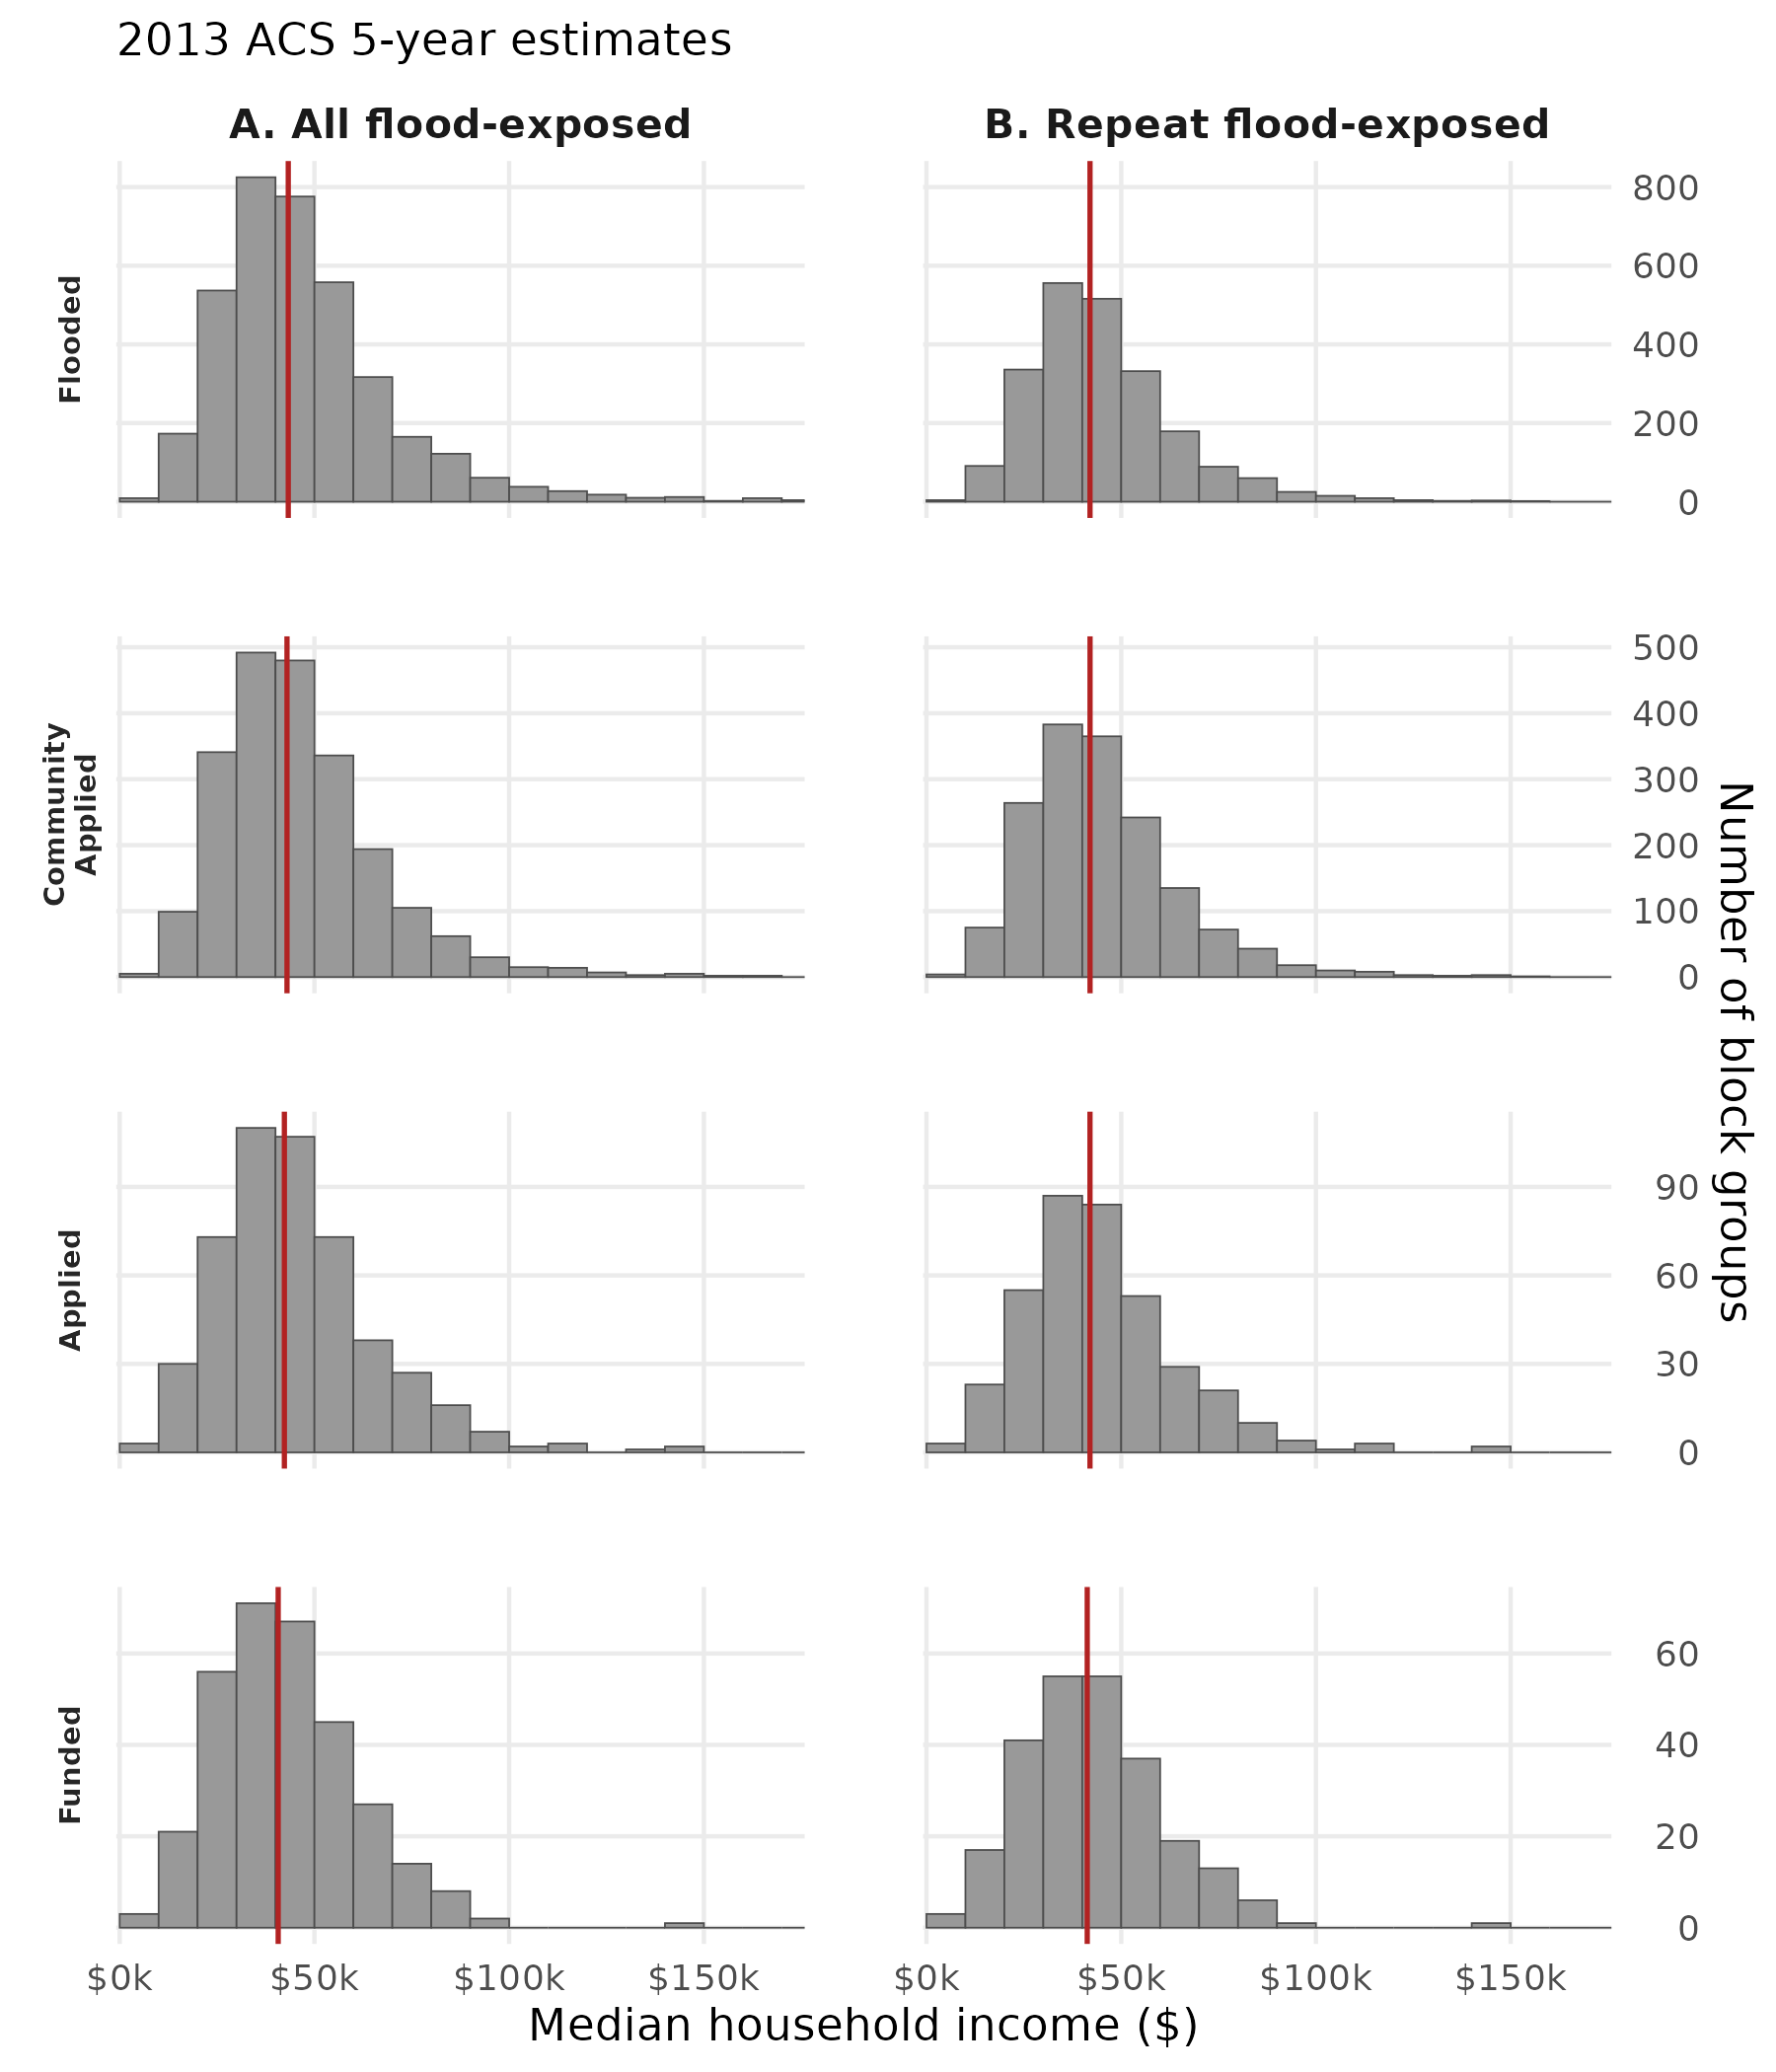
\includegraphics[width=1\linewidth,height=\textheight,keepaspectratio]{figures/fig5a_income.png}

}

\caption{\label{fig-si-income}\textbf{Block-group median household
income across the HMA pipeline.} Distribution of block-group median
household income (2013 ACS 5-year estimates) for block groups containing
at least one residential parcel reaching each pipeline stage. Panel A
shows all flood-exposed parcels; Panel B is restricted to repeat-flooded
parcels (those exposed to more than one of the 78 modeled events).
Stages from top to bottom: Flooded, Community Applied, Applied, Funded.
Red vertical lines mark stage medians. The x-axis is truncated at
\$175,000 for readability.}

\end{figure}%

\begin{figure}

\centering{

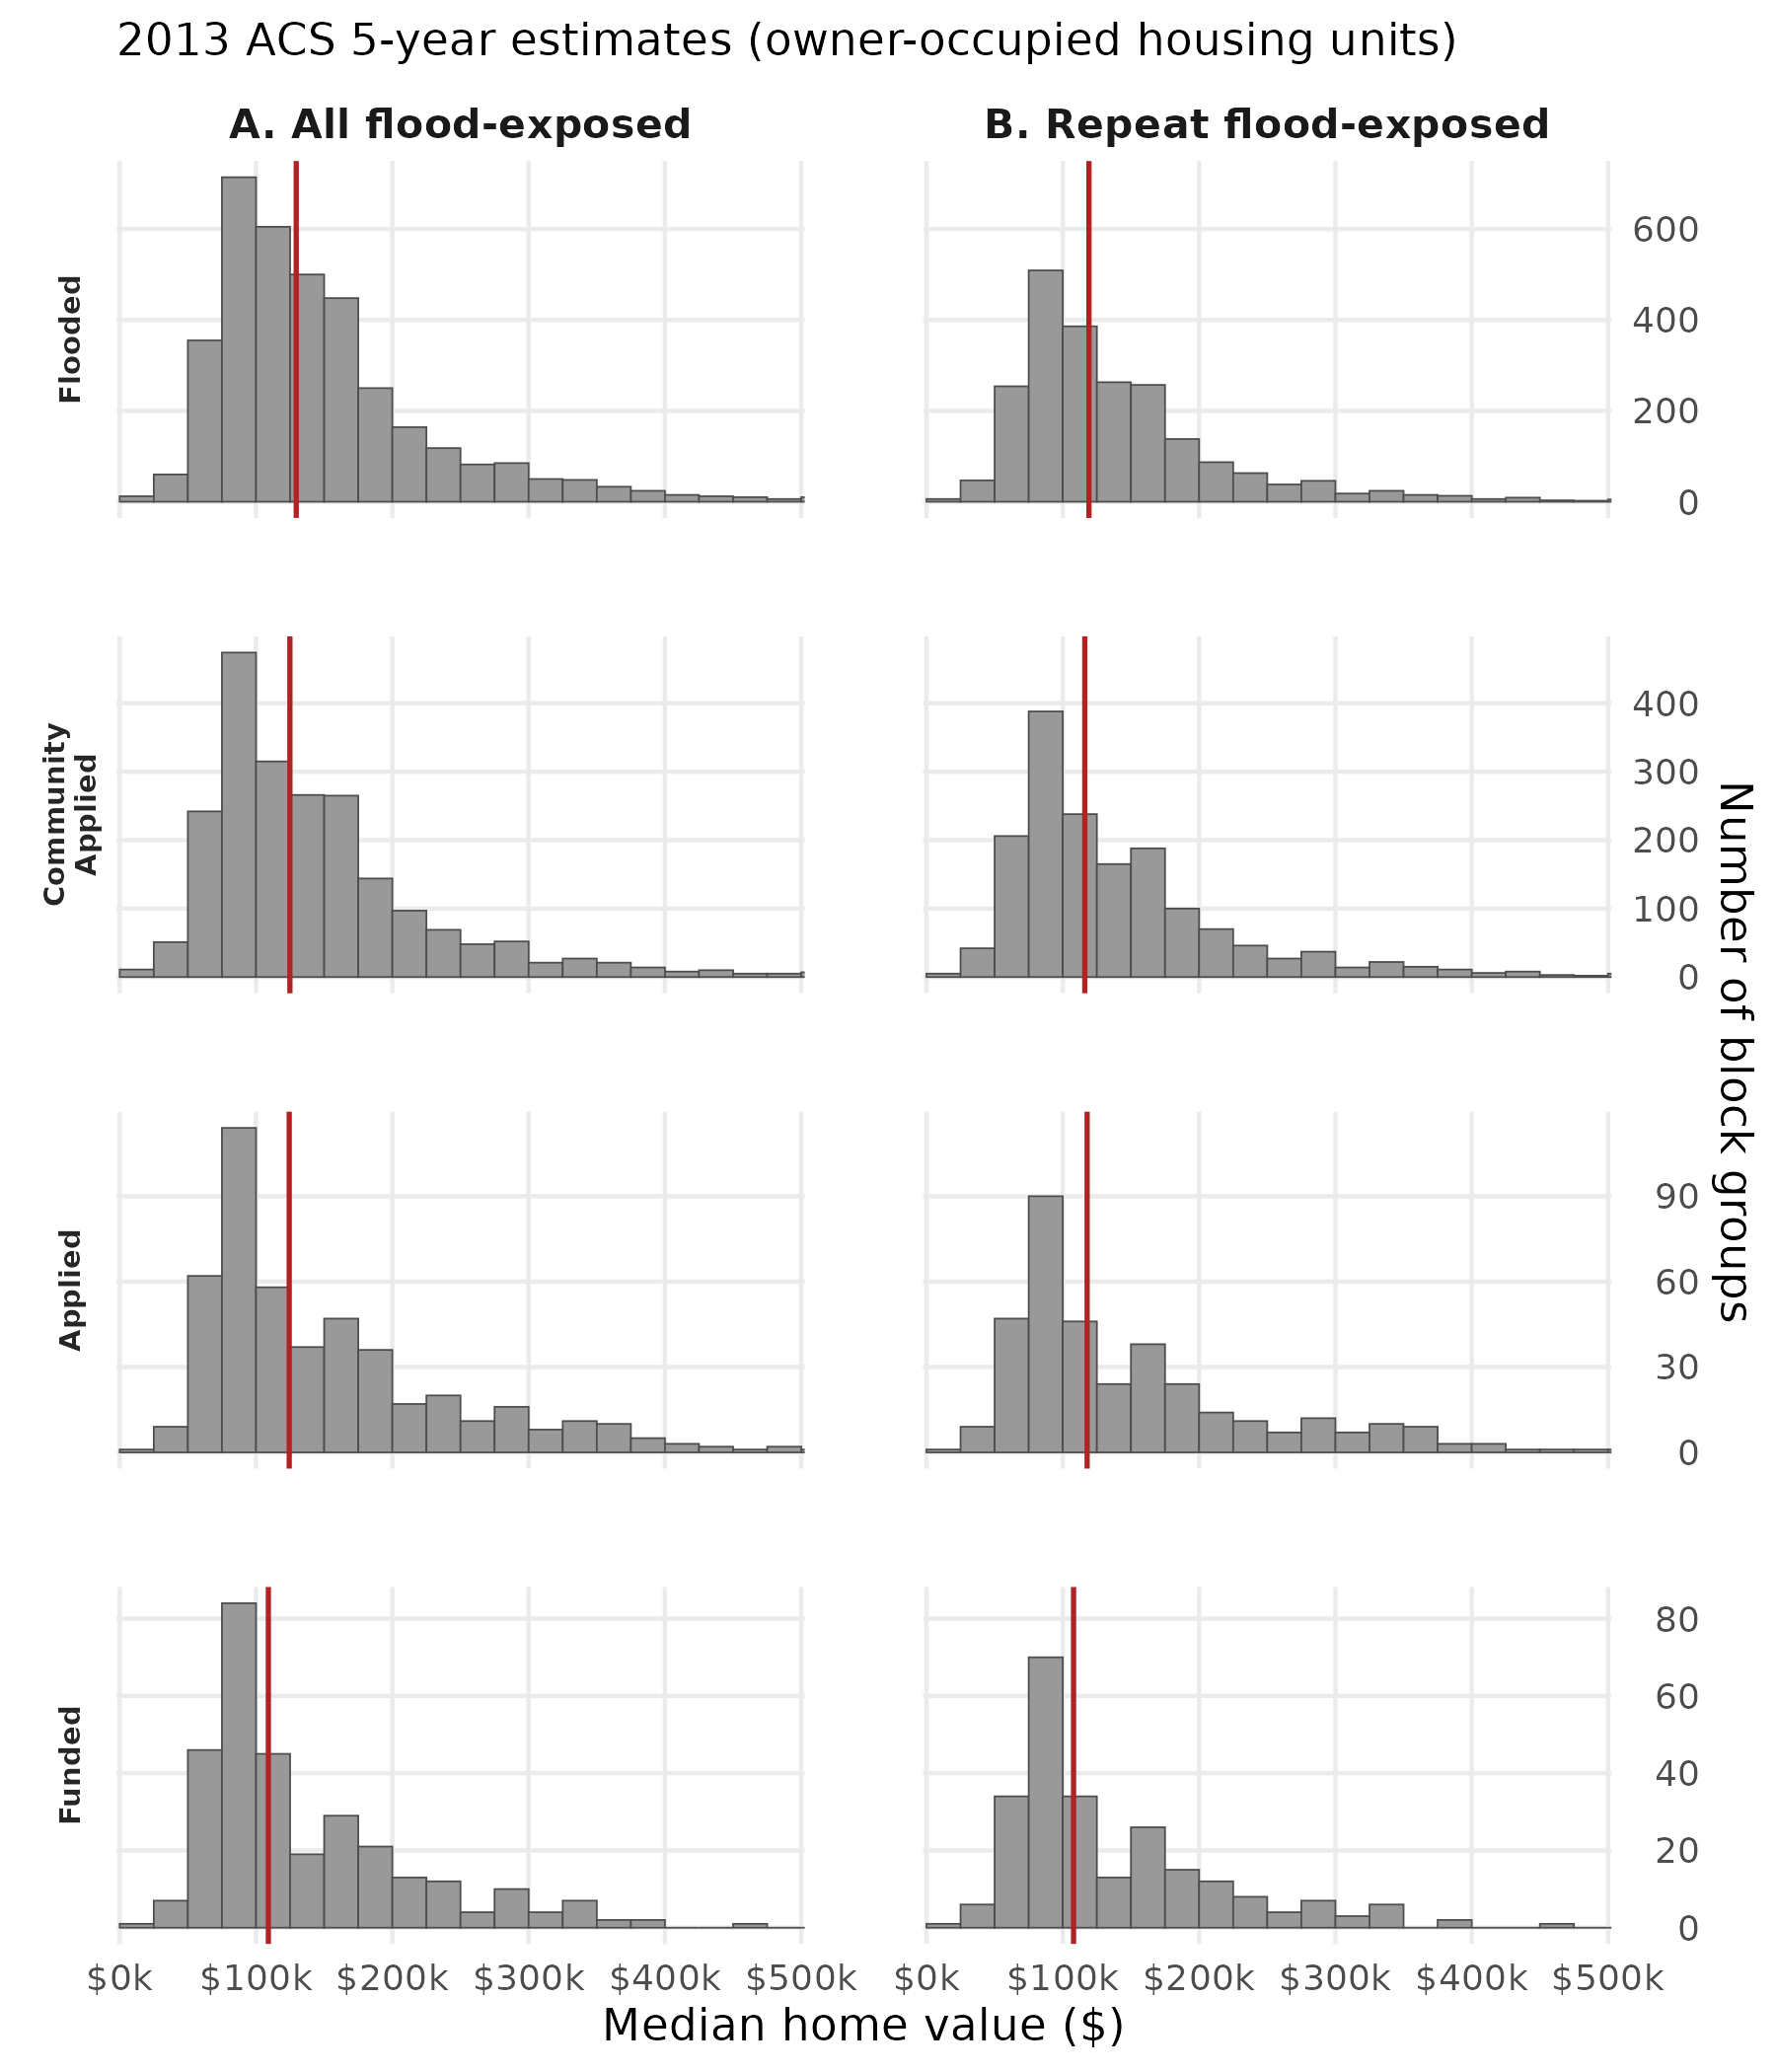
\includegraphics[width=1\linewidth,height=\textheight,keepaspectratio]{figures/fig5b_home_value.png}

}

\caption{\label{fig-si-homevalue}\textbf{Block-group median home value
across the HMA pipeline.} Distribution of block-group median home value
for owner-occupied housing (2013 ACS 5-year estimates) for block groups
containing at least one residential parcel reaching each pipeline stage.
Panel A shows all flood-exposed parcels; Panel B is restricted to
repeat-flooded parcels. Stages from top to bottom: Flooded, Community
Applied, Applied, Funded. Red vertical lines mark stage medians. The
x-axis is truncated at \$500,000 for readability.}

\end{figure}%

\subsection*{S2. Race and economic correlation in the study
area}\label{s2.-race-and-economic-correlation-in-the-study-area}
\addcontentsline{toc}{subsection}{S2. Race and economic correlation in
the study area}

\begin{figure}

\centering{

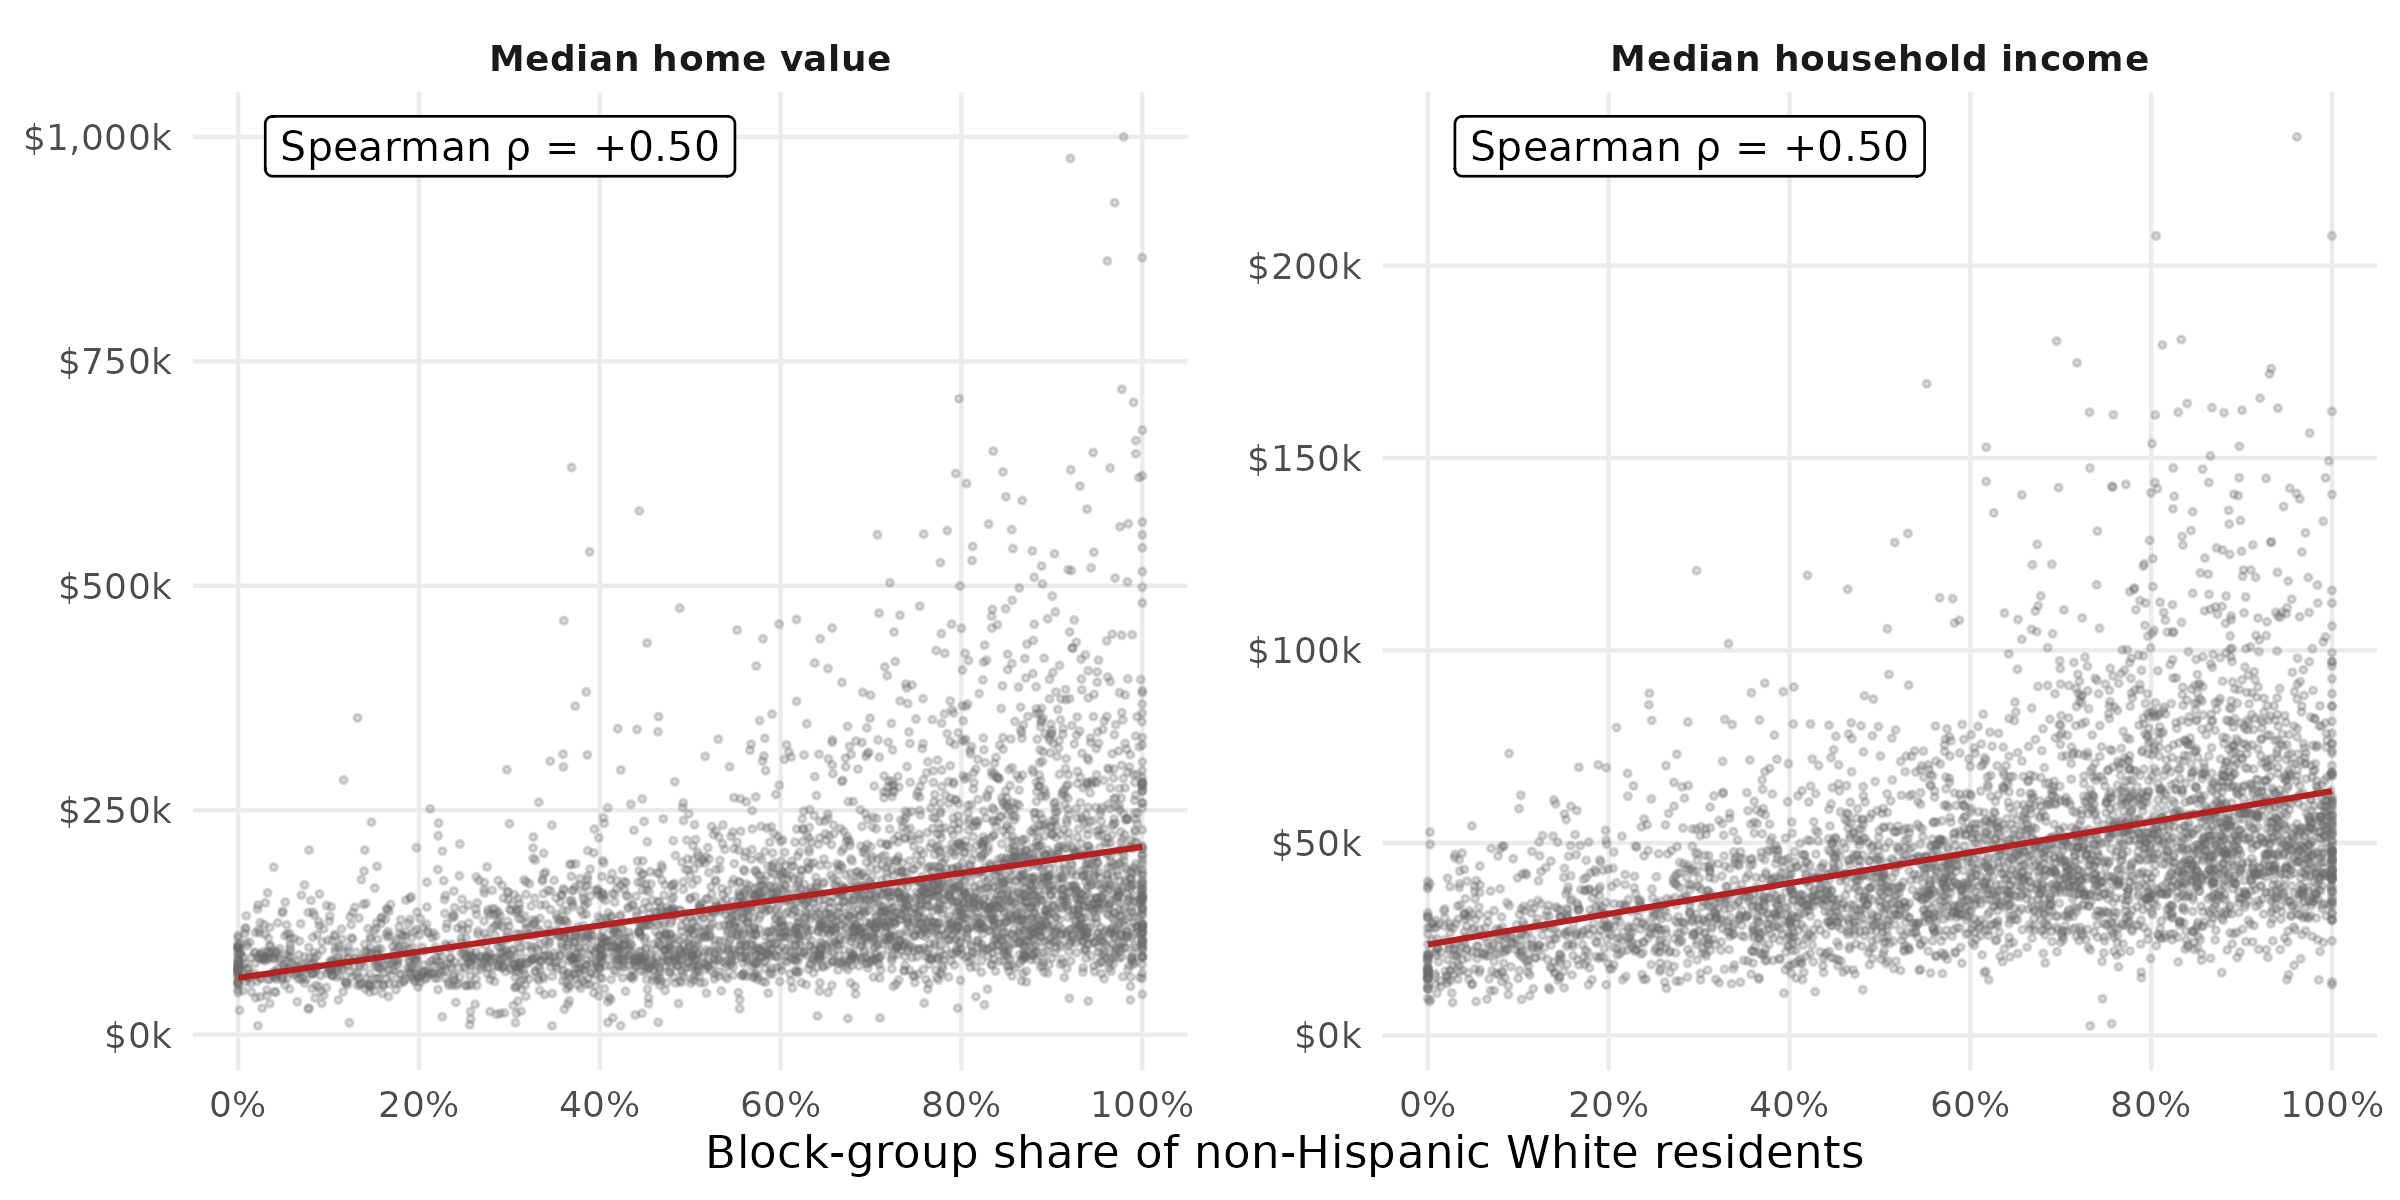
\includegraphics[width=1\linewidth,height=\textheight,keepaspectratio]{figures/figS1_race_value_correlation.png}

}

\caption{\label{fig-si-race-value}\textbf{Block-group correlation
between race and economic indicators across the study area.} Block-group
share of non-Hispanic White residents plotted against median home value
(left) and median household income (right), using 2013 American
Community Survey 5-year estimates for the 4,384 study-area block groups
with complete data. Red lines show ordinary least squares fits; Spearman
rank correlations are reported in each panel.}

\end{figure}%

\subsection*{S3. Buyouts versus elevations across all and repeat-flooded
funded
parcels}\label{s3.-buyouts-versus-elevations-across-all-and-repeat-flooded-funded-parcels}
\addcontentsline{toc}{subsection}{S3. Buyouts versus elevations across
all and repeat-flooded funded parcels}

The main-text comparison of buyouts and elevations
(Figure~\ref{fig-mit-type} in main text) restricts to the ``all funded''
subset. The figures below replicate that comparison while also showing
the repeat-flooded subset (Panel B), to verify that the buyout-elevation
divergence is not driven by event-specific dynamics.

\begin{figure}

\centering{

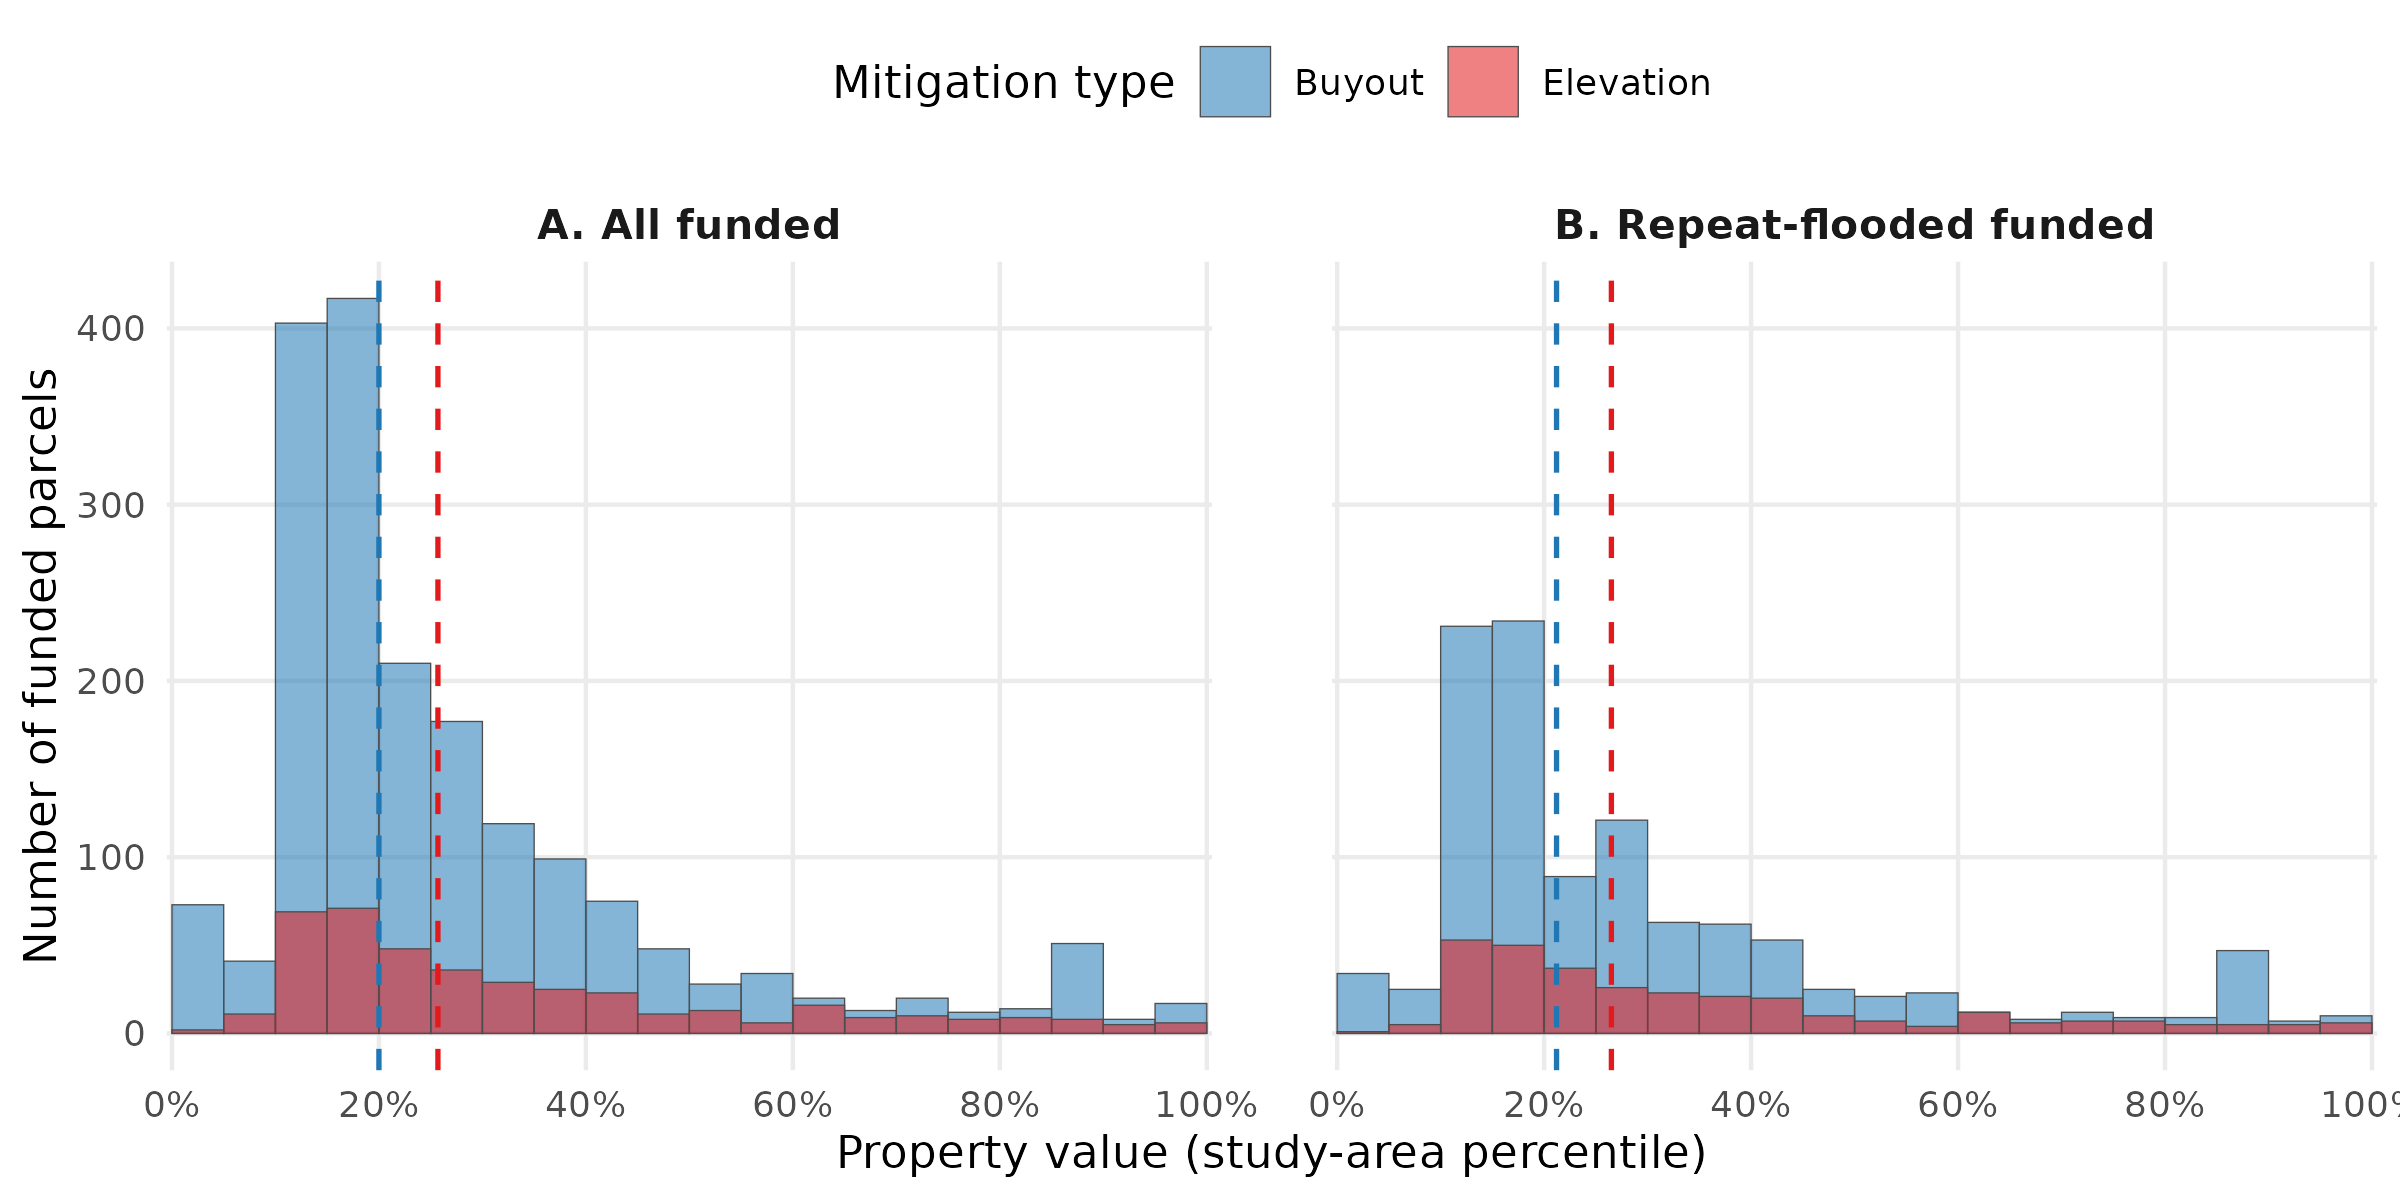
\includegraphics[width=1\linewidth,height=\textheight,keepaspectratio]{figures/figS2_mit_type_value.png}

}

\caption{\label{fig-si-mit-value}\textbf{Property value distributions by
mitigation type, all funded versus repeat-flooded.} Study-area
property-value percentile distributions for funded parcels classified as
buyouts (blue) versus elevations (red). Panel A includes all funded
parcels with a classified project type; Panel B restricts to
repeat-flooded funded parcels. Dashed vertical lines mark within-group
medians. Two-sample Kolmogorov-Smirnov tests indicate the distributions
differ significantly in both panels (Panel A: D = 0.141, p \textless{}
0.001; Panel B: D = 0.135, p \textless{} 0.001).}

\end{figure}%

\begin{figure}

\centering{

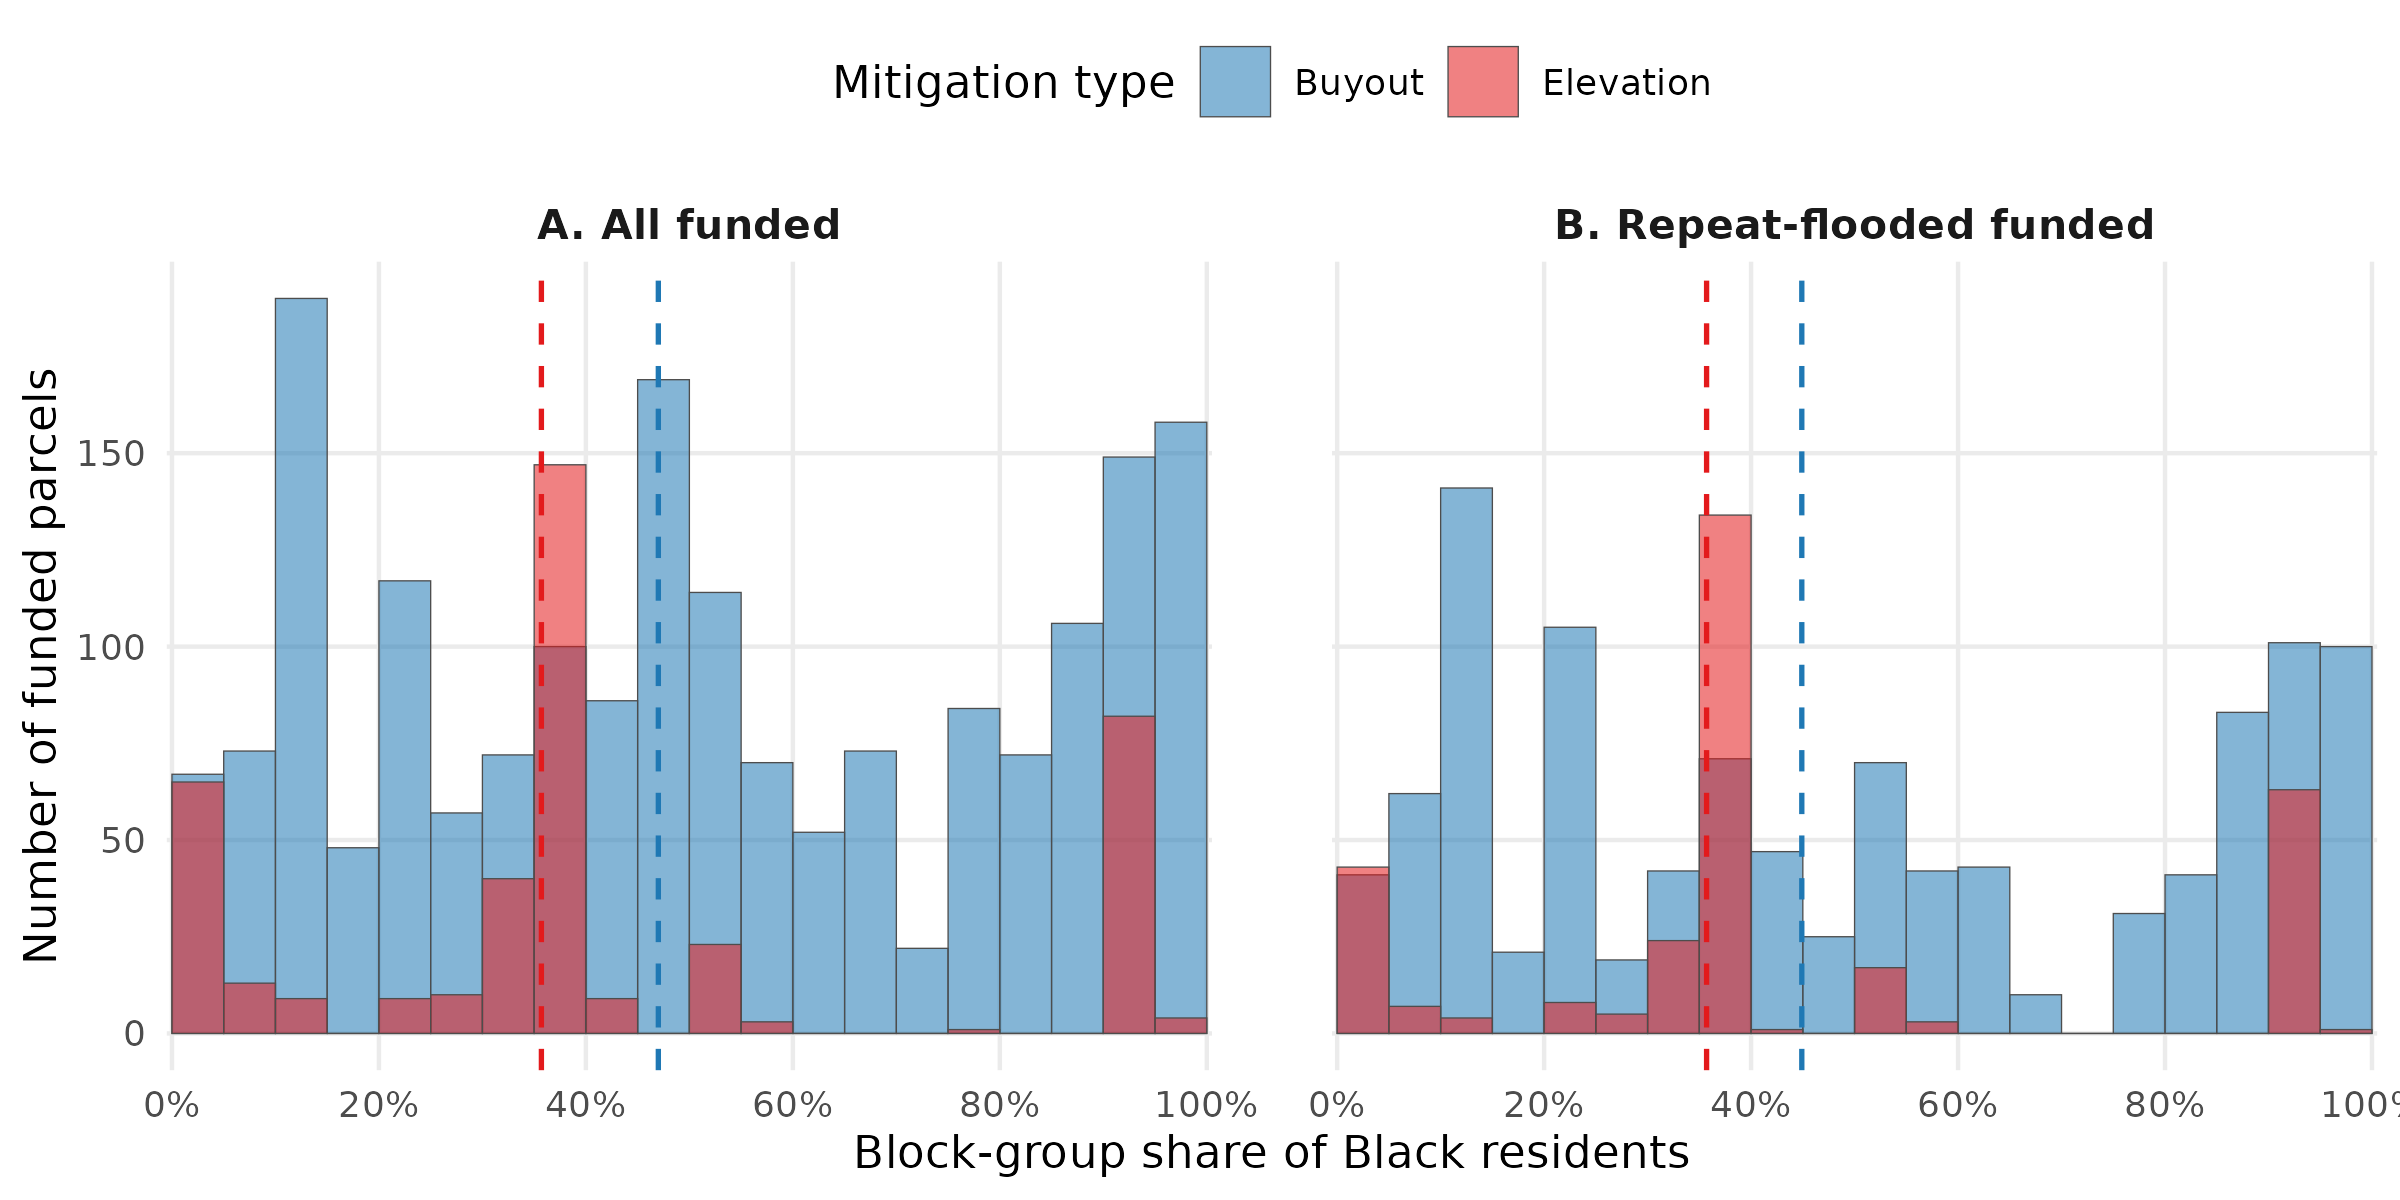
\includegraphics[width=1\linewidth,height=\textheight,keepaspectratio]{figures/figS3_mit_type_black.png}

}

\caption{\label{fig-si-mit-black}\textbf{Neighborhood racial composition
by mitigation type, all funded versus repeat-flooded.} Block-group share
of Black residents (2013 ACS) for funded parcels classified as buyouts
(blue) versus elevations (red). Panel A includes all funded parcels with
a classified project type; Panel B restricts to repeat-flooded funded
parcels. Dashed vertical lines mark within-group medians.
Kolmogorov-Smirnov tests indicate the distributions differ significantly
in both panels (Panel A: D = 0.366, p \textless{} 0.001; Panel B: D =
0.32, p \textless{} 0.001), with buyouts consistently located in block
groups with higher Black population shares.}

\end{figure}%

\subsection*{S4. Sensitivity to high-uncertainty
events}\label{s4.-sensitivity-to-high-uncertainty-events}
\addcontentsline{toc}{subsection}{S4. Sensitivity to high-uncertainty
events}

Garcia et al. \citeyearpar{garciaReconstructingRepetitiveFlood2025} flag
seven of the 78 events as having unusually high ratios of
modeled-flooded buildings to NFIP claims (more than 20 buildings per
claim), indicating greater uncertainty in those event reconstructions.
We rebuilt the full flooded-to-funded pipeline excluding these seven
events to verify that our headline findings do not depend on them; the
excluded events are listed in
\href{https://doi.org/10.1029/2025EF006026}{Garcia et al.} and
reproduced in Table~\ref{tbl-sens-funnel}.

Excluding the seven events meaningfully reduces the flooded-residential
population (202,623 → 172,329 parcels, −14.9\%) and the eligible
population (141,253 → 129,685 parcels, −8.2\%, attributable largely to
TS Allison, the only declared event among the seven). However, only 78
of the 3,432 funded parcels in the baseline are tied exclusively to the
excluded events, so the funded population shifts only marginally (3,432
→ 3,354 parcels, −2.3\%).

The pinch point at the application stage is essentially identical across
scenarios: 4.3\% of properties in applying communities themselves apply
under both the baseline and the 71-event sensitivity. Median
funded-stage demographics and property values shift by less than half a
percentage point: median NH White share moves from 60.0\% to 59.6\%,
median Black share from 26.1\% to 26.3\%, and median study-area
property-value percentile from the 23rd to the 23rd. Two-sample
Kolmogorov-Smirnov tests of flooded-versus-funded block-group racial
distributions remain highly significant under the sensitivity scenario,
with D-statistics slightly larger than the baseline (NH White: D = 0.146
versus 0.131, p \textless{} 0.001; Black: D = 0.162 versus 0.151, p
\textless{} 0.001). The headline pinch-point and demographic-composition
findings are therefore robust to the exclusion of the seven
high-uncertainty events.

\begin{longtable}[]{@{}lrrr@{}}
\caption{Pipeline funnel under baseline (all 78 events) and sensitivity
(71 events, excluding the seven events Garcia et al.~flag as having
unusually high uncertainty).}\label{tbl-sens-funnel}\tabularnewline
\toprule\noalign{}
Stage & Baseline (78 events) & Sensitivity (71 events) & Change \\
\midrule\noalign{}
\endfirsthead
\toprule\noalign{}
Stage & Baseline (78 events) & Sensitivity (71 events) & Change \\
\midrule\noalign{}
\endhead
\bottomrule\noalign{}
\endlastfoot
Flooded & 202,623 & 172,329 & −14.9\% \\
Eligible & 141,253 & 129,685 & −8.2\% \\
Community Applied & 132,828 & 121,713 & −8.4\% \\
Applied & 5,746 & 5,259 & −8.5\% \\
Funded & 3,432 & 3,354 & −2.3\% \\
\end{longtable}

\begin{longtable}[]{@{}lrr@{}}
\caption{Funded-stage demographics and statistical tests under baseline
vs sensitivity. All KS test p-values \textless{} 0.001 in both
scenarios.}\label{tbl-sens-medians}\tabularnewline
\toprule\noalign{}
Metric & Baseline & Sensitivity \\
\midrule\noalign{}
\endfirsthead
\toprule\noalign{}
Metric & Baseline & Sensitivity \\
\midrule\noalign{}
\endhead
\bottomrule\noalign{}
\endlastfoot
Median property value (study-area percentile) & 23rd & 23rd \\
Median NH White block-group share & 60.0\% & 59.6\% \\
Median Black block-group share & 26.1\% & 26.3\% \\
KS test: NH White (D-statistic) & 0.131 & 0.146 \\
KS test: Black (D-statistic) & 0.151 & 0.162 \\
\end{longtable}





\end{document}
